\documentclass[conference]{IEEEtran}
\IEEEoverridecommandlockouts
\usepackage[T1]{fontenc}
\usepackage{amsmath,amssymb}
\usepackage{mathptmx}
\usepackage{microtype}
\usepackage{graphicx}
\usepackage{booktabs}
\usepackage{xurl}
\usepackage[hidelinks]{hyperref}
\usepackage{amsopn}
\usepackage{float}
\usepackage{placeins}
\usepackage{morefloats}
\usepackage{afterpage}
\graphicspath{{figures/}}
\setlength{\textfloatsep}{10pt plus 2pt minus 2pt}
\setlength{\dbltextfloatsep}{10pt plus 2pt minus 2pt}
\renewcommand{\topfraction}{0.95}
\renewcommand{\bottomfraction}{0.95}
\renewcommand{\dbltopfraction}{0.95}
\renewcommand{\textfraction}{0.02}
% Single-column float pages only need to be 70% full; full-width figures get a
% page of their own only if they fill 90% of it, otherwise they share a page with text.
\renewcommand{\floatpagefraction}{0.7}
\renewcommand{\dblfloatpagefraction}{0.9}
\setcounter{topnumber}{5}
\setcounter{bottomnumber}{5}
\setcounter{totalnumber}{10}
\setcounter{dbltopnumber}{4}
% Stack floats from the top of float-only pages with a fixed gap, instead of
% spreading them over the whole page, and tighten the gap between stacked floats.
\makeatletter
\setlength{\@fptop}{0pt}
\setlength{\@fpsep}{8pt}
\setlength{\@fpbot}{0pt plus 1fil}
\setlength{\@dblfptop}{0pt}
\setlength{\@dblfpsep}{8pt}
\setlength{\@dblfpbot}{0pt plus 1fil}
\makeatother
\setlength{\floatsep}{8pt plus 2pt minus 2pt}
\setlength{\dblfloatsep}{8pt plus 2pt minus 2pt}
\DeclareMathOperator{\sign}{sign}
\newcommand{\vect}[1]{\mathbf{#1}}

\begin{document}

\title{ECSE 551 Assignment 1: Lasso and ElasticNet Regression, SVM and MLP Classifiers, and S\&P\,500 Return Prediction}

\author{\IEEEauthorblockN{William Charron-Boyle, Radman Jamalshirpanjeh, Brandon Ku, Jack McDonald}
\IEEEauthorblockA{Department of Electrical and Computer Engineering, McGill University, Montr\'eal, QC, Canada}}

\maketitle

\begin{abstract}
We analysed two benchmark datasets, implemented four models from scratch and applied simple models to stock return prediction. Using only NumPy and gradient descent, we implemented Lasso and ElasticNet regression with soft thresholding, a one-vs-rest support vector machine (SVM) and a one-hidden-layer multilayer perceptron (MLP), and compared them with scikit-learn's \texttt{LinearRegression} and \texttt{RandomForestClassifier}. On Diabetes, \texttt{LinearRegression} had the lowest test mean squared error (2538.7), with our Lasso and ElasticNet close behind (2586.0 and 2611.8) while shrinking the large opposing weights that least squares gives to correlated features. On Digits, the MLP was most accurate (98.0\%), ahead of the random forest (97.0\%) and the SVM (96.7\%). For next-day volatility-adjusted S\&P\,500 returns, Lasso, random forest and MLP regressors retrained yearly on a rolling window all had positive test Sharpe ratios (1.7--4.0), and sentiment data helped only slightly.
\end{abstract}

\section{Introduction}
This assignment has three tasks. Task~1 explores two scikit-learn datasets. The Diabetes dataset~\cite{skAPI,efron} has 442 patients with ten baseline variables (age, sex, body mass index \texttt{bmi}, blood pressure \texttt{bp} and six serum measurements \texttt{s1}--\texttt{s6}) and a continuous measure of disease progression after one year as the target. The Digits dataset~\cite{skAPI} has 1797 handwritten digits stored as $8\times8$ images, giving 64 pixel features and a label from 0 to 9.

Task~2 asks us to implement two regression models, ElasticNet and Lasso, and two classifiers, a multiclass support vector machine (SVM) and a multilayer perceptron (MLP), using only NumPy~\cite{harris} and gradient descent, and to compare them with scikit-learn's~\cite{sklearn} \texttt{LinearRegression} and \texttt{RandomForestClassifier}, with a 70/30 train/test split and hyperparameters chosen by cross-validation.

Task~3 uses daily returns of S\&P\,500 stocks from 1980 to 2013, plus sentiment data for 2009--2015, to predict each stock's volatility-adjusted return for tomorrow from information available today, using Lasso, random forest and MLP regressors from scikit-learn. We evaluate the predictions with the Sharpe ratio, the profit-and-loss (PnL) curve, the cumulative rank correlation and the average holding period.

In short, regularisation does not improve the test error on Diabetes but makes the coefficients easier to interpret, the non-linear models beat the linear SVM on Digits by a small margin, and on the stock data simple reversal and low-volatility signals give a weak but consistent edge out of sample, although the best models change their positions almost every day.

\section{Datasets}
\subsection{Diabetes and Digits}
Neither dataset needed cleaning: there are no missing, infinite or duplicated values, and every value lies in a valid range (Diabetes target 25--346, Digits pixels integers 0--16). Scikit-learn already centres the Diabetes features and gives them a common scale (standard deviation $\approx0.048$), whereas the raw units vary widely (e.g.\ 19--79 for age). We used them as provided, since a common scale is what the $\ell_1$ and $\ell_2$ penalties need to treat all features equally; this scaling was computed on all 442 patients, a leak of test information that we consider negligible.

All Diabetes features are unimodal except the binary \texttt{sex} (Fig.~\ref{fig:diab_hist}); \texttt{bmi}, \texttt{s3} and \texttt{s4} are right-skewed, \texttt{s4} is nearly discrete, and none has heavy tails. The points outside the box-plot whiskers (Fig.~\ref{fig:diab_box}; 31 of the 442 patients have at least one) are plausible health measurements, so we kept them. Two feature pairs are strongly correlated (Fig.~\ref{fig:diab_corr}), \texttt{s1}--\texttt{s2} ($r=0.90$) and \texttt{s3}--\texttt{s4} ($r=-0.74$), which is a good reason to try regularisation. The feature--target relationships are roughly linear but noisy (Fig.~\ref{fig:diab_scatter}, with the Pearson $r$ in each title): \texttt{bmi} ($r=0.59$) and \texttt{s5} ($r=0.57$) are the strongest, \texttt{sex} ($r=0.04$) and \texttt{s2} ($r=0.17$) the weakest.

% Box plots and correlation matrix side by side in one full-width float,
% so every float in this section is the same width and they pack together.

\begin{figure*}[!tp]
\centering
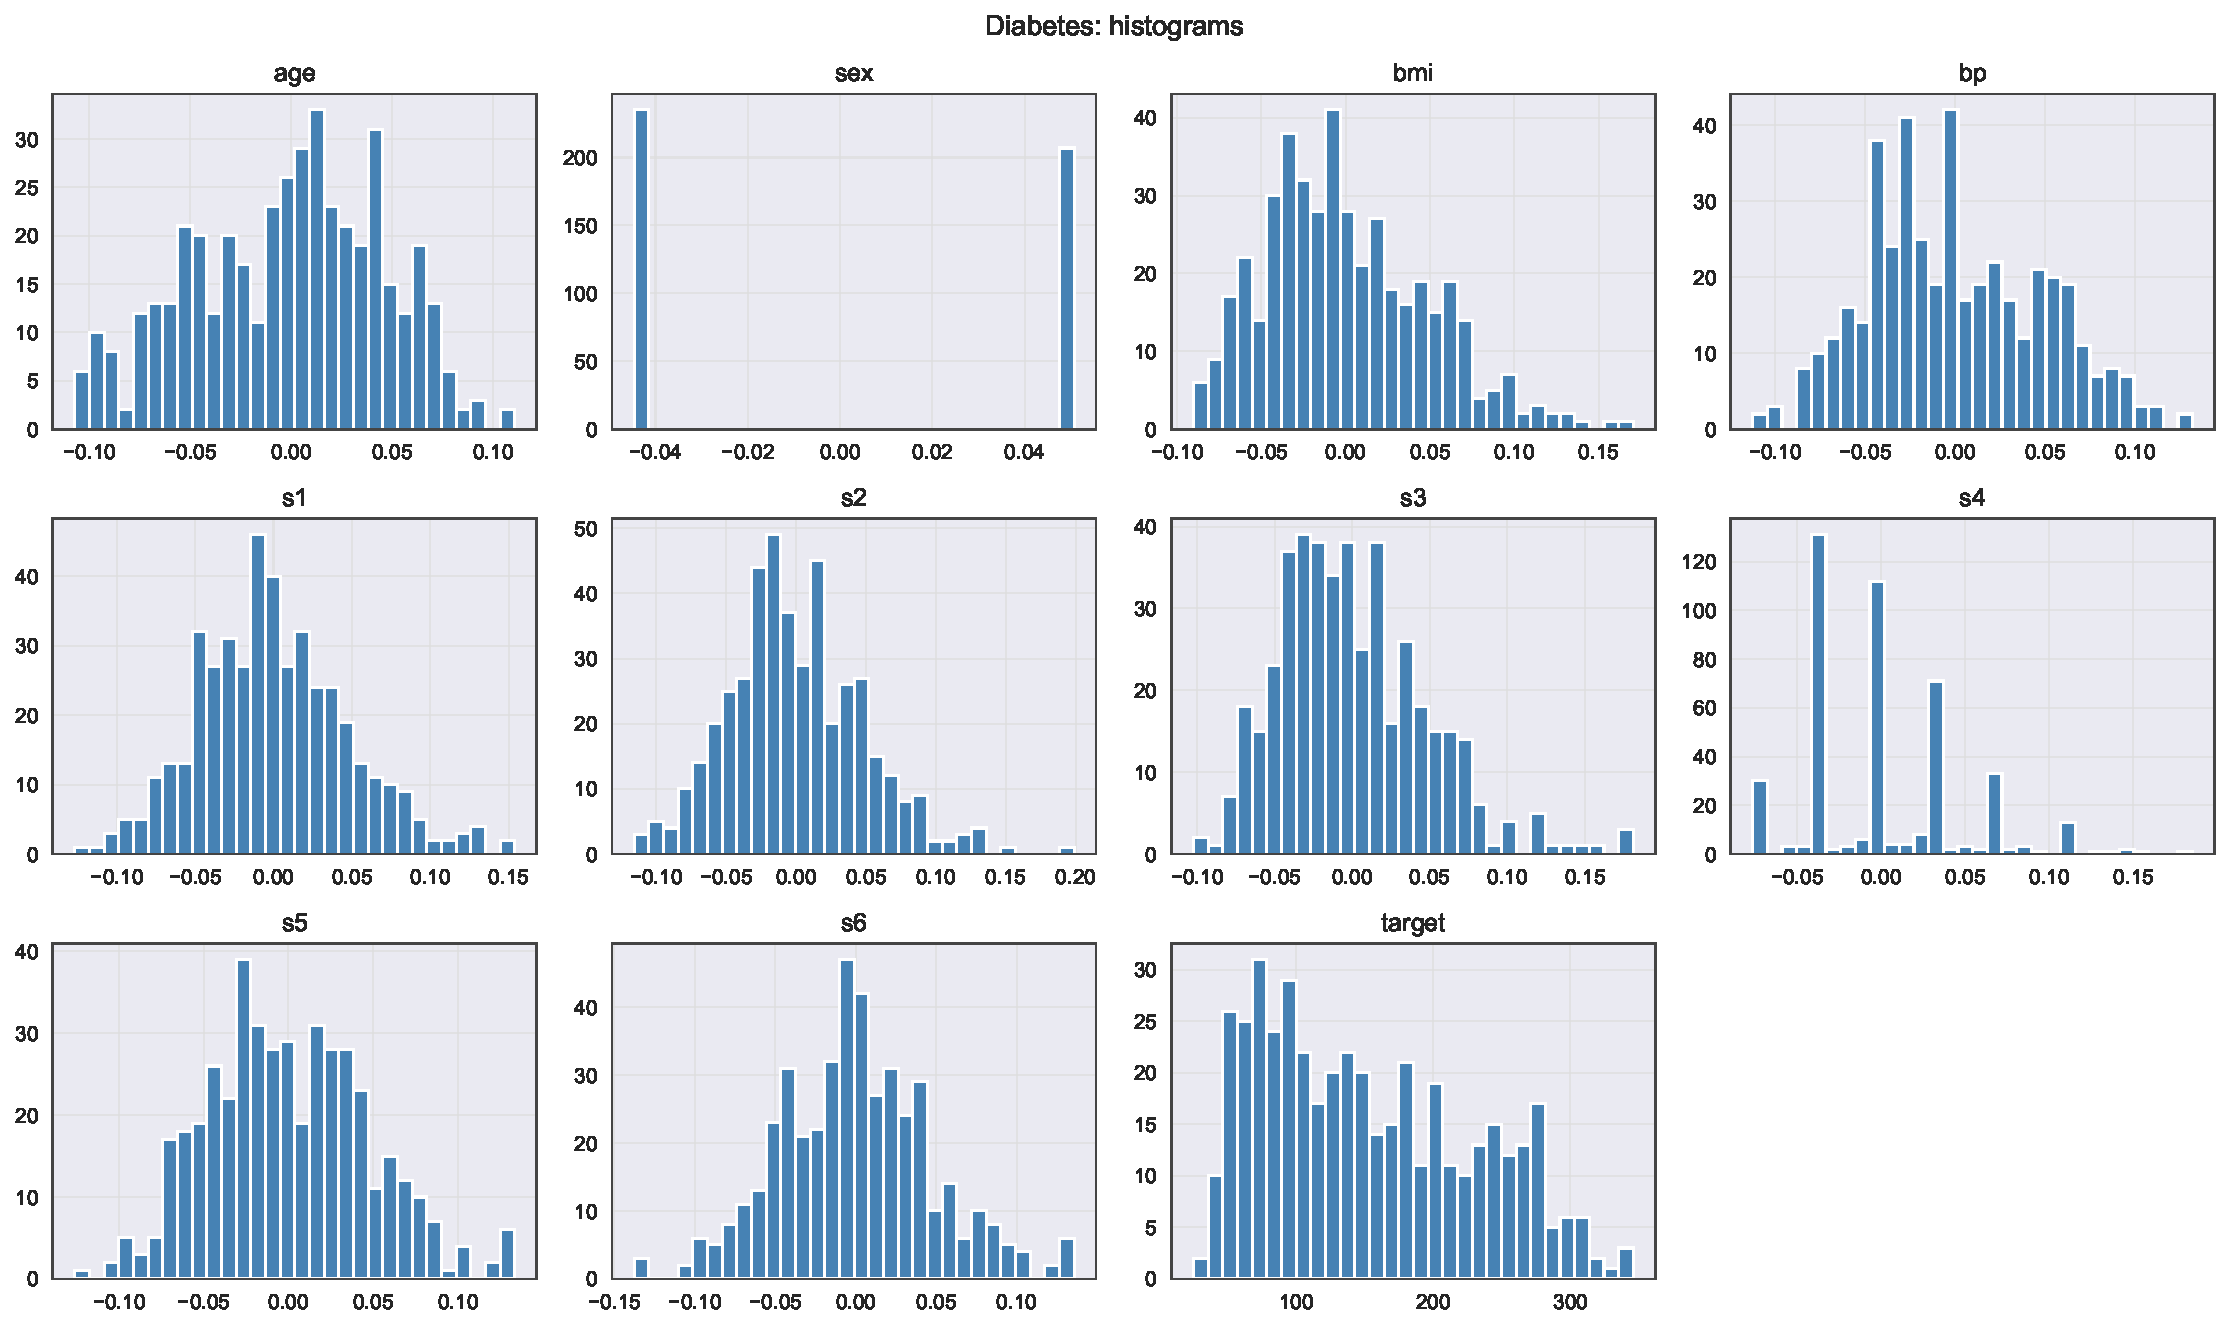
\includegraphics[width=0.9\textwidth]{diab_hist.pdf}
\caption{Distributions of the Diabetes features and target. The \texttt{sex} feature is binary, \texttt{s4} is nearly discrete, and the other features are unimodal and mostly slightly right-skewed.}
\label{fig:diab_hist}
\end{figure*}

\begin{figure*}[!tp]
\centering
\begin{minipage}[t]{0.55\textwidth}
\vspace{0pt}
\centering
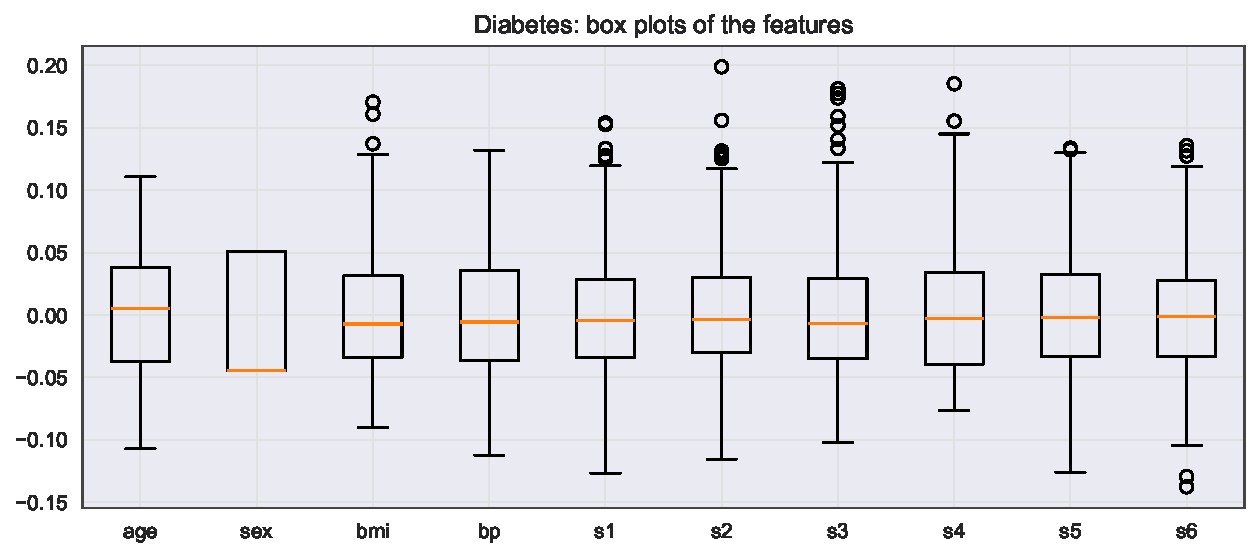
\includegraphics[width=\linewidth]{diabetes_boxplots.pdf}
\caption{Box plots of the ten Diabetes features (scikit-learn-scaled units). Outliers are plausible values and were kept.}
\label{fig:diab_box}
\end{minipage}\hfill
\begin{minipage}[t]{0.43\textwidth}
\vspace{0pt}
\centering
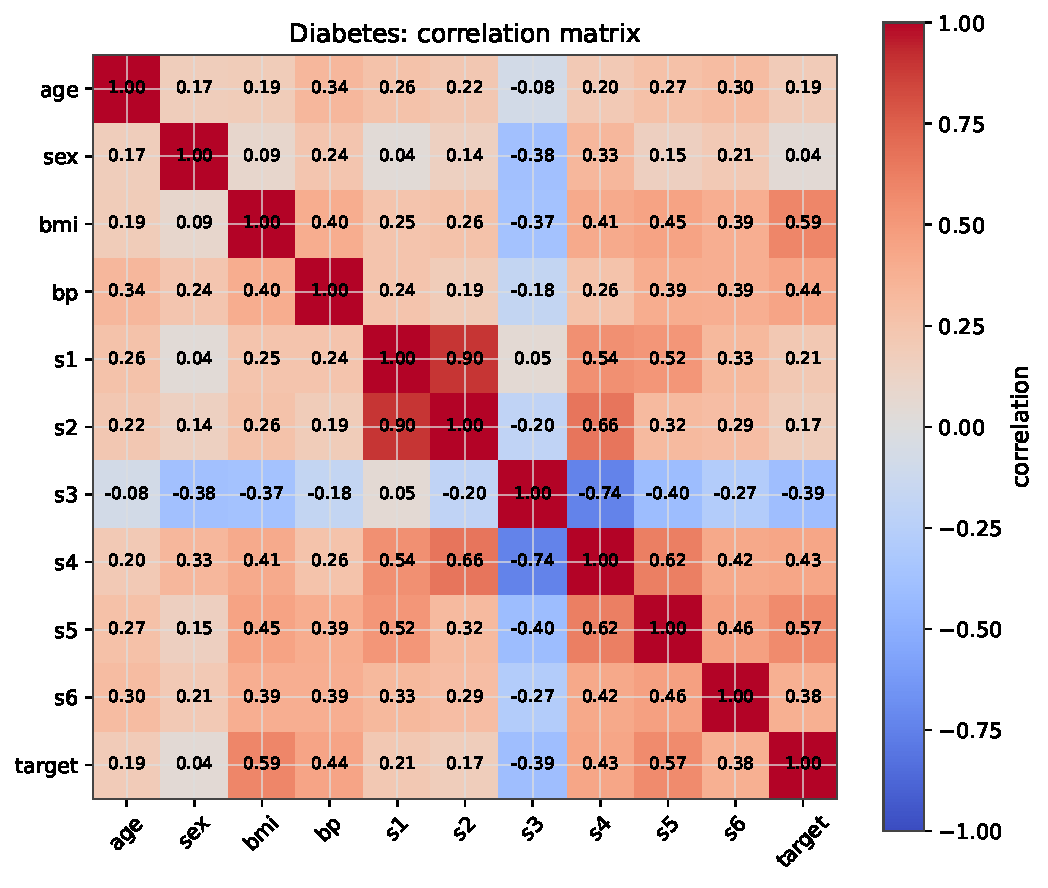
\includegraphics[width=0.92\linewidth]{diab_corr.pdf}
\caption{Pearson correlation matrix of the Diabetes data. Note the strongly correlated pairs \texttt{s1}--\texttt{s2} and \texttt{s3}--\texttt{s4}.}
\label{fig:diab_corr}
\end{minipage}
\end{figure*}

\begin{figure*}[!tp]
\centering
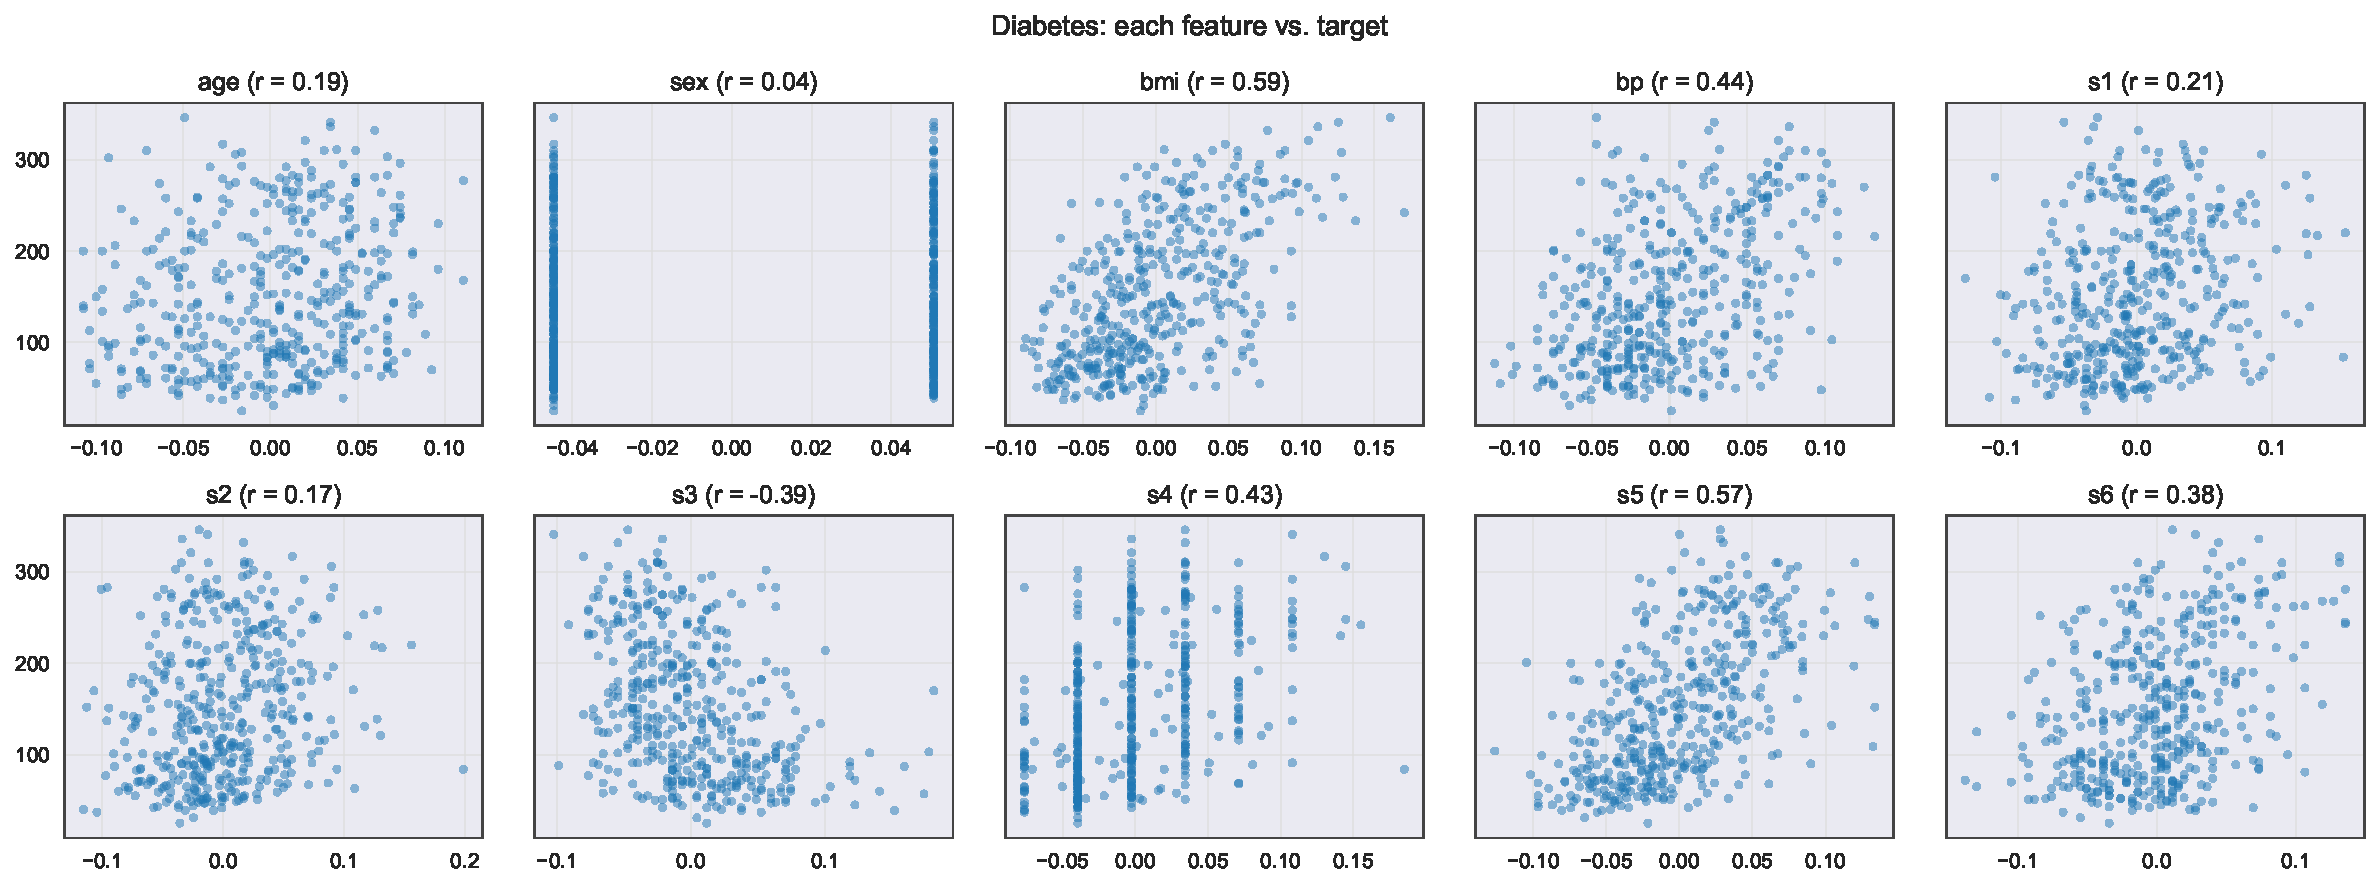
\includegraphics[width=0.95\textwidth,height=0.3\textheight,keepaspectratio]{diabetes_feature_vs_target.pdf}
\caption{Each Diabetes feature against the target, with the Pearson $r$ shown in each panel title. The features \texttt{bmi} and \texttt{s5} are the most linearly related to the target.}
\label{fig:diab_scatter}
\end{figure*}

\begin{figure*}[!tp]
\centering
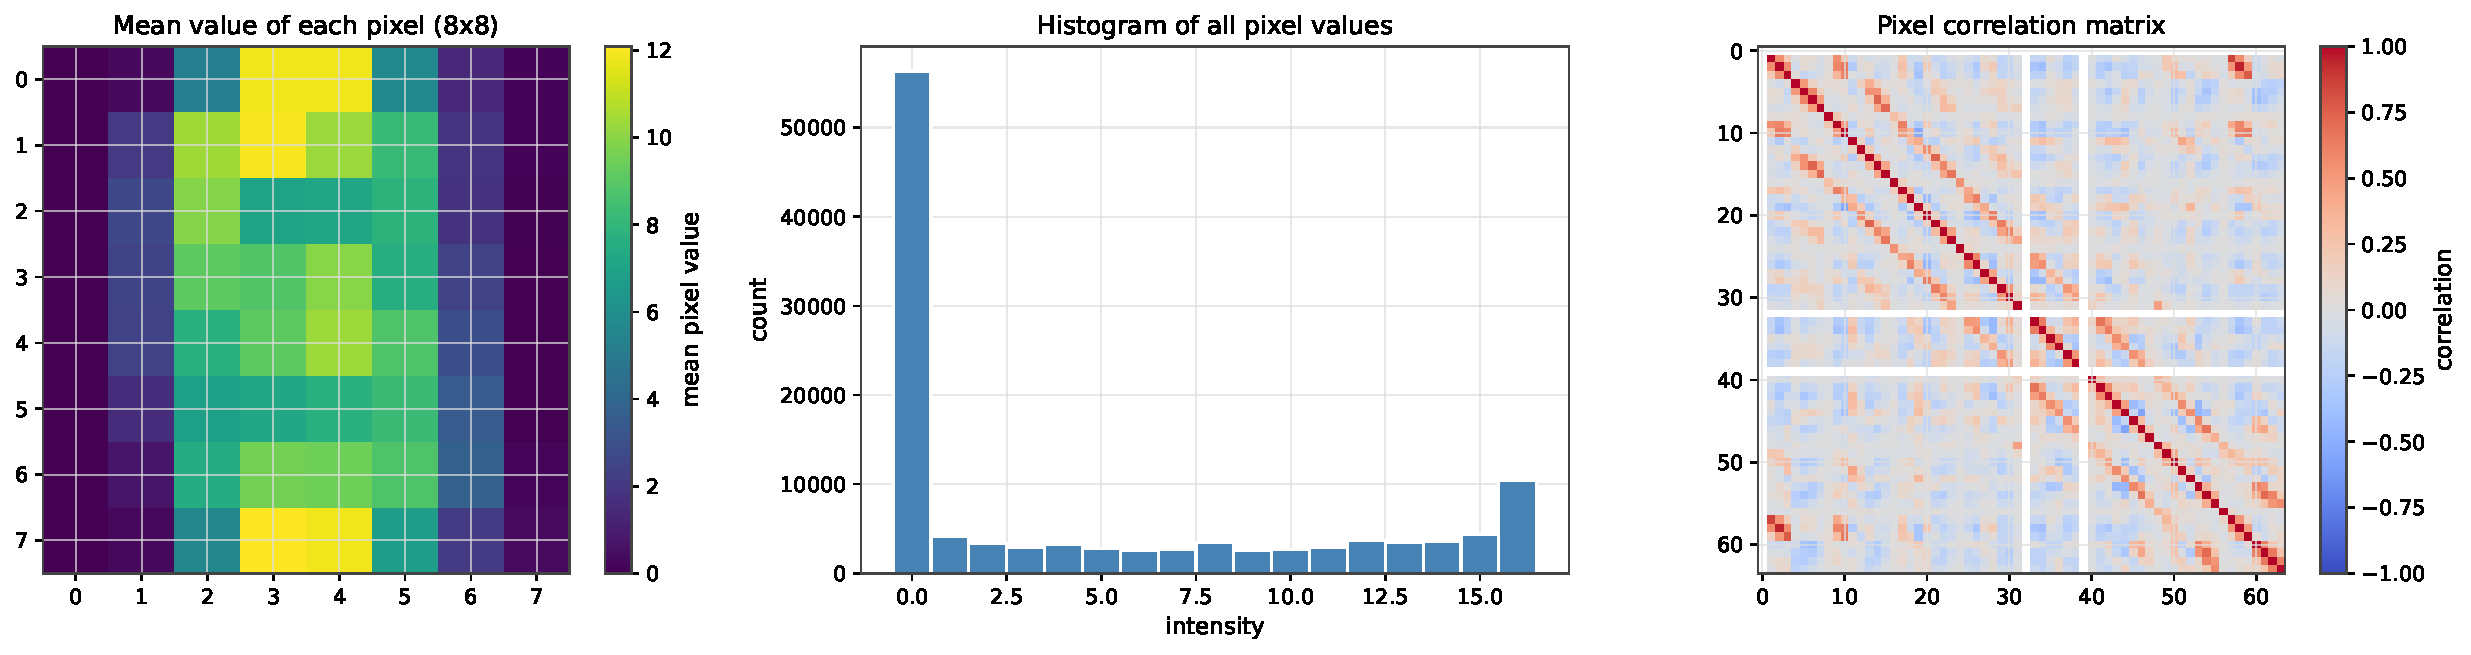
\includegraphics[width=\textwidth,height=0.45\textheight,keepaspectratio]{digits_stats.pdf}
\caption{Digits: mean of each pixel, the histogram of all pixel values, and the correlation matrix of all pixel values.}
\label{fig:dig_stats}
\end{figure*}

The ten Digits classes are balanced (174--183 images each), so accuracy is a fair metric. Pixel values are strongly bimodal, with about half at 0 (background) and a second peak at 16 (fully inked), and pixels 0, 32 and 39 are always 0. Edge pixels are almost always 0, while central pixels span the full range, so the pixel means run from 0 to about 12 and the standard deviations from 0 to 6.5 (Fig.~\ref{fig:dig_stats}). We therefore standardised the pixels with training-split statistics. Neighbouring pixels are modestly correlated (bands next to the diagonal of the correlation matrix).

\subsection{\texorpdfstring{S\&P\,500 Returns and Sentiment}{S\&P 500 Returns and Sentiment}}
\label{sec:spdata}
The return file covers 8577 trading days and 1335 stocks. The membership file marks between 489 and 500 index members on each day, and no member has a missing return. We only make and evaluate predictions for stocks that are members on day $t$. The Psychsignal sentiment data start in July 2009, but they cover few members: on average, 57 members per day in 2009, rising to 233 in 2013.

\section{Methodology}
\label{sec:method}
The equations in this section follow the course lecture notes~\cite{notes}. All from-scratch models are trained with gradient descent, $\theta_{t+1}=\theta_t-\eta\,\vect{g}_t$, where $\vect{g}_t$ is the gradient (or subgradient) of the loss and $\eta$ is the learning rate. Hyperparameters are chosen by 5-fold cross-validation (CV), which estimates the risk of a setting $\lambda$ as $R^{\mathrm{cv}}_\lambda=\frac{1}{K}\sum_{k=1}^{K}R_0\big(\hat\theta_\lambda(\mathcal{D}_{-k}),\mathcal{D}_k\big)$ with $K=5$~\cite{notes}, i.e.\ the average score over five train-on-four, test-on-one splits. The Diabetes data are split by a NumPy permutation seeded with 42 (309 training and 133 test patients), with CV folds from a second seeded permutation of the training rows. The Digits data are split by scikit-learn's \texttt{train\_test\_split} with \texttt{random\_state=42} (1257 training and 540 test images), and the three classifiers share the same five folds (\texttt{KFold}~\cite{skAPI}, shuffled with random state 42).

\subsection{Regression Models}
Let $\vect{X}$ be the $m\times n$ feature matrix (for Diabetes, the scikit-learn-scaled features), $\vect{y}$ the targets, $\vect{w}$ the weights and $b$ the bias, which is never penalised. We report the mean squared error, $\mathrm{MSE}=\frac{1}{m}\sum_i(y_i-\hat y_i)^2$, and the coefficient of determination, $R^2=1-\sum_i(y_i-\hat y_i)^2/\sum_i(y_i-\bar y)^2$, which is the fraction of the target variance explained by the model.

\textit{Linear regression.} \texttt{LinearRegression} minimises the training sum of squared errors with an unpenalised intercept. Its solution is the ordinary least squares (OLS) estimate $\hat{\vect{w}}=(\vect{X}^\top\vect{X})^{-1}\vect{X}^\top\vect{y}$ for centred $\vect{X}$ and $\vect{y}$~\cite{notes}, and it serves as our baseline.

\textit{Lasso.} Lasso~\cite{tibshirani} adds an $\ell_1$ penalty to the squared error, which pushes some weights to exactly zero:
\begin{equation}
\min_{\vect{w},b}\ \frac{1}{2m}\|\vect{y}-(\vect{X}\vect{w}+b\vect{1})\|_2^2+\lambda\|\vect{w}\|_1 .
\label{eq:lasso}
\end{equation}
Since $|w_j|$ has no derivative at zero, we used the proximal gradient method from Lecture~8: each iteration takes a gradient step on the squared error and then soft-thresholds each weight,
\begin{equation}
\vect{v}=\vect{w}+\tfrac{\eta}{m}\vect{X}^\top\vect{e},\quad w_j\leftarrow S_{\eta\lambda}(v_j)=\sign(v_j)\max\big(|v_j|-\eta\lambda,\,0\big),
\label{eq:soft}
\end{equation}
where $\vect{e}=\vect{y}-\vect{X}\vect{w}-b\vect{1}$ is the residual. Weights smaller than $\eta\lambda$ in magnitude become exactly zero, and all others move towards zero by $\eta\lambda$.

\textit{ElasticNet.} ElasticNet~\cite{zou} combines both penalties, with overall strength $\lambda$ and $\ell_1$ ratio $\rho\in[0,1]$:
\begin{equation}
\min_{\vect{w},b}\ \frac{1}{2m}\|\vect{y}-(\vect{X}\vect{w}+b\vect{1})\|_2^2+\lambda\Big(\rho\|\vect{w}\|_1+\frac{1-\rho}{2}\|\vect{w}\|_2^2\Big) .
\label{eq:enet}
\end{equation}
so $\rho=1$ gives Lasso and $\rho=0$ ridge. The $\ell_2$ term makes correlated features share their weight, whereas Lasso tends to keep only one of them~\cite{notes}. We used the same method, with the $\ell_2$ penalty in the gradient step and the $\ell_1$ part in the threshold:
\begin{equation}
\vect{v}=\vect{w}+\frac{\eta}{m}\vect{X}^\top\vect{e}-\eta\lambda(1-\rho)\vect{w},\quad w_j\leftarrow S_{\eta\lambda\rho}(v_j),
\label{eq:enet-update}
\end{equation}
so ElasticNet also produces exact zeros, whenever $|v_j|\le\eta\lambda\rho$. In both models the unpenalised bias takes a plain gradient step, $b\leftarrow b+\frac{\eta}{m}\vect{1}^\top\vect{e}$.

\textit{Learning rate and tuning.} Gradient descent needs $\eta$ below 2 divided by the largest curvature of the smooth objective. For the weights, this curvature is the largest eigenvalue $L$ of $\vect{X}^\top\vect{X}/m$ plus $\lambda(1-\rho)$. Because the scaled features are small, $L\approx8.2\cdot10^{-3}$, so this bound ($\eta<2/L\approx240$) is loose, and the binding limit is the unpenalised bias, whose curvature of 1 requires $\eta<2$. The same scaling makes the smallest eigenvalue only $1.9\cdot10^{-5}$, along a direction mixing mainly the collinear \texttt{s1} and \texttt{s2} (with some \texttt{s3} and \texttt{s5}), where gradient descent converges slowly (Section~\ref{sec:reg}). A sweep over $\eta\in\{10^{-3},10^{-2},10^{-1},1,1.5,2\}$ at $\lambda=0.01$, $\rho=0.5$ showed that $\eta=1.5$ converges fastest within 500 iterations. For the regularisation path we used $\eta=1.5/\max(1,\,L+\lambda(1-\rho))$, 10\,000 iterations, 35 values of $\lambda\in[10^{-4},10]$ and $\rho\in\{0,0.25,0.5,0.75,1\}$, and selected $\lambda$ and $\rho$ by 5-fold CV MSE\@.

\subsection{Classification Models}
\textit{Multiclass SVM.} A binary SVM~\cite{cortes} uses the decision function $f(\vect{x})=\vect{w}^\top\vect{x}+w_0$ with labels $\tilde y_i\in\{-1,+1\}$. As shown in Lecture~8, the soft-margin SVM is equivalent to minimising the hinge loss with an $\ell_2$ penalty:
\begin{equation}
\min_{\vect{w},w_0}\ \frac12\|\vect{w}\|_2^2+\gamma\sum_{i=1}^{m}\max\big(0,\,1-\tilde y_i(\vect{w}^\top\vect{x}_i+w_0)\big).
\label{eq:hinge}
\end{equation}
Following the class template, we wrote the penalty as $\lambda\|\vect{w}\|^2$ and averaged the hinge losses, which is the same problem rescaled with $\gamma=1/(2\lambda m)$. Only the margin violators $S=\{i:\tilde y_i f(\vect{x}_i)<1\}$ contribute to the subgradient, giving the updates
\begin{equation}
\vect{w}\leftarrow\vect{w}-\eta\Big(2\lambda\vect{w}-\frac1m\sum_{i\in S}\tilde y_i\vect{x}_i\Big),\quad w_0\leftarrow w_0+\frac{\eta}{m}\sum_{i\in S}\tilde y_i .
\end{equation}
For ten classes, we trained one classifier per digit against all the others and predicted the digit with the highest score~\cite{notes}, searching $\eta$ from 0.001 to 3 and $\lambda$ from $10^{-4}$ to 1, then the number of iterations.

\textit{MLP.} Our MLP has one hidden layer of $H$ units with the rectified linear unit activation $\mathrm{ReLU}(a)=\max(a,0)$ and a softmax output $\mu_c=e^{a_c}/\sum_{c'}e^{a_{c'}}$, giving one probability per digit~\cite{notes}. We trained it with full-batch gradient descent on the cross-entropy, or negative log-likelihood (NLL), loss from Lecture~6:
\begin{equation}
\mathrm{NLL}(\theta)=-\frac{1}{m}\sum_{i=1}^{m}\sum_{c=1}^{10}y_{ic}\log\mu_{ic},
\label{eq:ce}
\end{equation}
where $y_{ic}$ is the one-hot label (from \texttt{OneHotEncoder}~\cite{skAPI}). Backpropagation (the chain rule, layer by layer) gives the output gradient $(\boldsymbol{\mu}-\vect{y})/m$, which is passed back through the ReLU, whose derivative is 1 for positive inputs and 0 otherwise. We searched $H$ from 8 to 512 and $\eta$ from 0.01 to 2, then the number of epochs.

\textit{Random forest.} A random forest~\cite{breiman} is an ensemble of decision trees. Each tree is grown on a bootstrap sample of the training data, and at each node it considers a random subset of the features and picks the split that most reduces the Gini impurity. Scikit-learn's version predicts the class with the highest probability averaged over the trees~\cite{skRF}; averaging partly independent trees reduces variance. We tuned the number of trees ($\{50,100,300\}$), the maximum depth ($\{\text{none},10,20\}$), the number of features per split ($\sqrt{n}$ or $\log_2 n$) and the minimum leaf size ($\{1,2\}$) with \texttt{GridSearchCV}~\cite{skAPI} on the same five folds. We compare the classifiers by accuracy, the fraction of test images whose predicted digit is correct, and by confusion matrices.

\subsection{Return Prediction}
\textit{Problem formulation.} We treat Task~3 as cross-sectional regression on the return, membership and sentiment data of Section~\ref{sec:spdata}: on each trading day $t$, for every S\&P\,500 member (about 500, well above the required 100), we predict its volatility-adjusted return for day $t+1$ from information available at the close of day $t$. Only the relative ordering of stocks matters for a market-neutral portfolio, so the target is demeaned across stocks each day. We train on data from 1981 to 2010, use 2001--2010 as the validation period for hyperparameters, and keep 2011--2013 as the test set. We evaluate with the Sharpe ratio, the PnL curve, the cumulative rank correlation and the average holding period (see \textit{Metrics}).

\textit{Volatility adjustment.} As described in the assignment, we track each stock's mean and variance with two exponentially weighted moving averages (EWMA): $\hat\mu_t=(1-\beta_2)r_t+\beta_2\hat\mu_{t-1}$ and $\hat\sigma_t^2=(1-\beta_1)(r_t-\hat\mu_t)^2+\beta_1\hat\sigma_{t-1}^2$, with $\beta_1=0.97$ and $\beta_2=0.99$. We drop each stock's first 60 days as burn-in. The adjusted return is $\tilde r_t=r_t/\hat\sigma_{t-1}$.

\begin{figure*}[!tp]
\centering
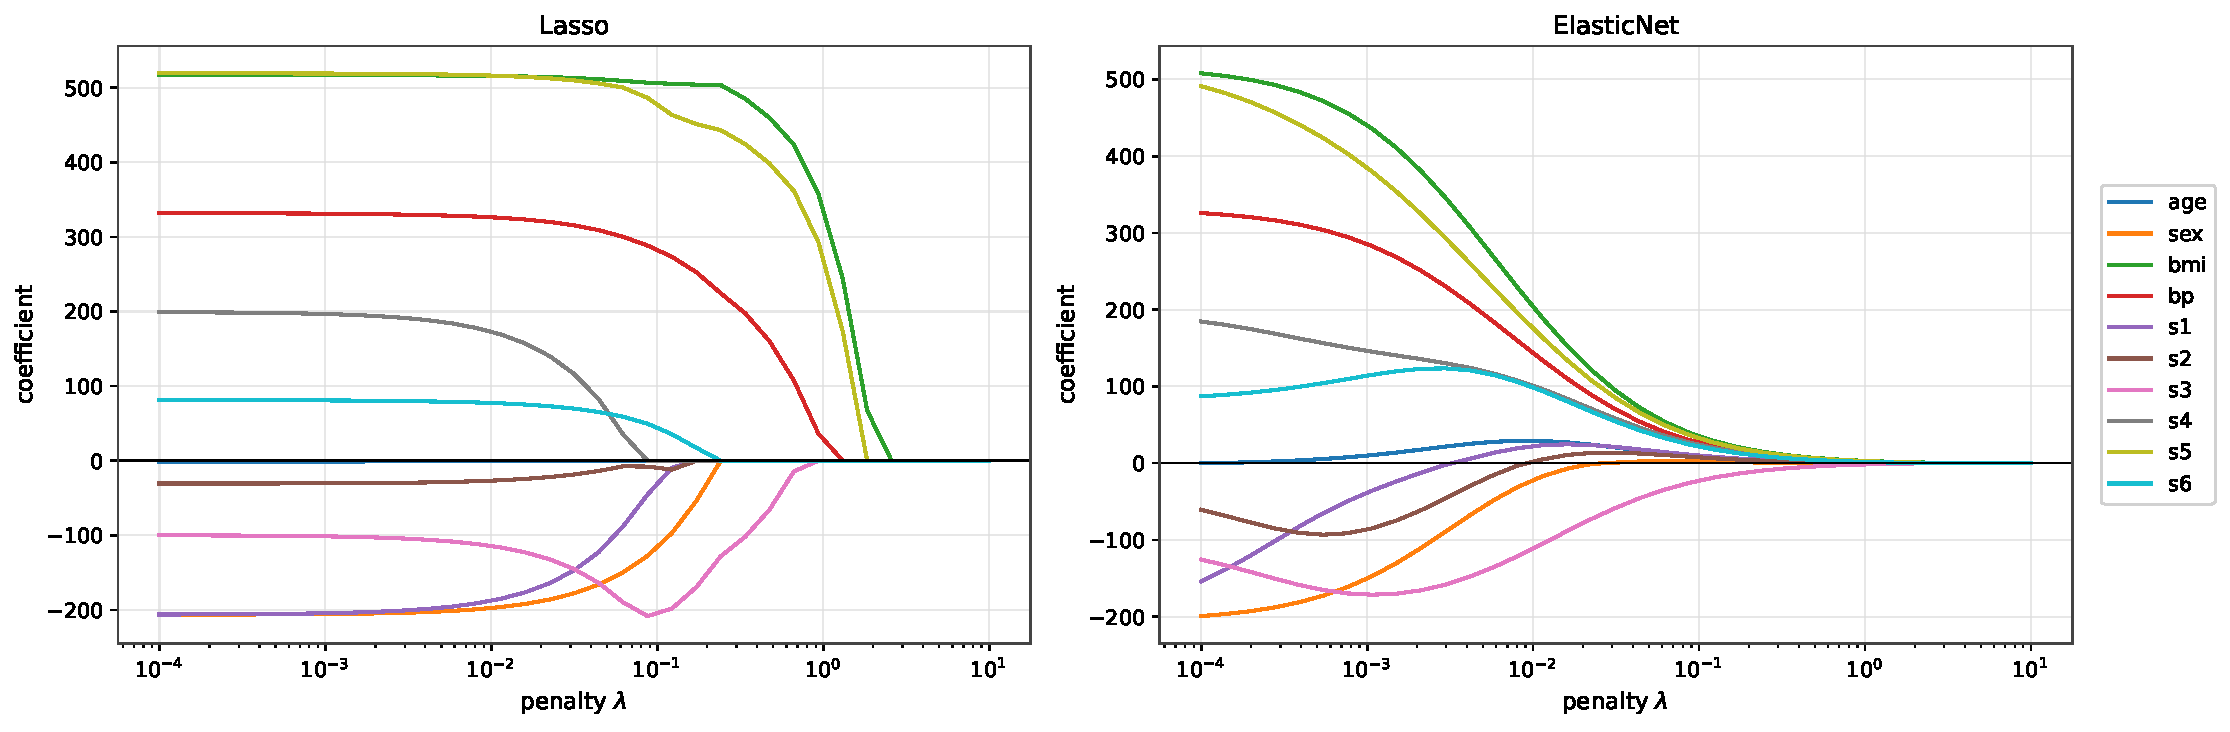
\includegraphics[width=\textwidth]{paths.pdf}
\caption{Coefficient paths for Lasso (left) and ElasticNet at $\rho=0.5$ (right) as the penalty $\lambda$ increases. Lasso drops weights to exactly zero one at a time; ElasticNet shrinks them more gradually and zeroes them only at larger $\lambda$. At the smallest $\lambda$, the weights have not yet converged to the OLS solution (Section~\ref{sec:reg}).}
\label{fig:paths}
\end{figure*}

\textit{Exploratory analysis.} Volatility adjustment brings the standard deviation of member returns from 0.024 to about 1.06, and the adjusted series look roughly stationary. We built six features on day $t$: the last return (\texttt{rev1}), the mean return over 5, 20 and 60 days (\texttt{rev5}, \texttt{mom20}, \texttt{mom60}), a longer-term mean that skips the latest month (\texttt{mom250}) and the log volatility (\texttt{vol}). Their average daily Spearman correlations with the next-day return are all below 0.03 in magnitude (Table~\ref{tab:ic}). The signs show short-term reversal, long-term momentum and a preference for low-volatility stocks, and \texttt{rev1} changed sign around 1992, so the relationships change over time.

\begin{table}[t]
\centering
\caption{Average daily rank correlation with the next-day return}
\label{tab:ic}
\footnotesize\setlength{\tabcolsep}{3.5pt}
\begin{tabular}{lcccccc}
\toprule
 & rev1 & rev5 & mom20 & mom60 & mom250 & vol\\
\midrule
1981--2000 & 0.001 & $-0.029$ & $-0.018$ & $-0.011$ & 0.012 & $-0.016$\\
2001--2010 & $-0.021$ & $-0.014$ & $-0.009$ & $-0.005$ & 0.011 & $-0.011$\\
\bottomrule
\end{tabular}
\end{table}

\textit{Data processing and leakage control.} Adjusted returns are clipped to $\pm5$, and each day every feature is z-scored across member stocks and clipped to $\pm3$. To prevent look-ahead, $\tilde r_t$ uses the volatility of day $t-1$, every feature on day $t$ uses only returns up to day $t$, a model used in year $Y$ is trained only on earlier data (dropping the last training day, so that no training target overlaps the prediction period), and all hyperparameters are chosen on 2001--2010.

\begin{figure*}[!tp]
\centering
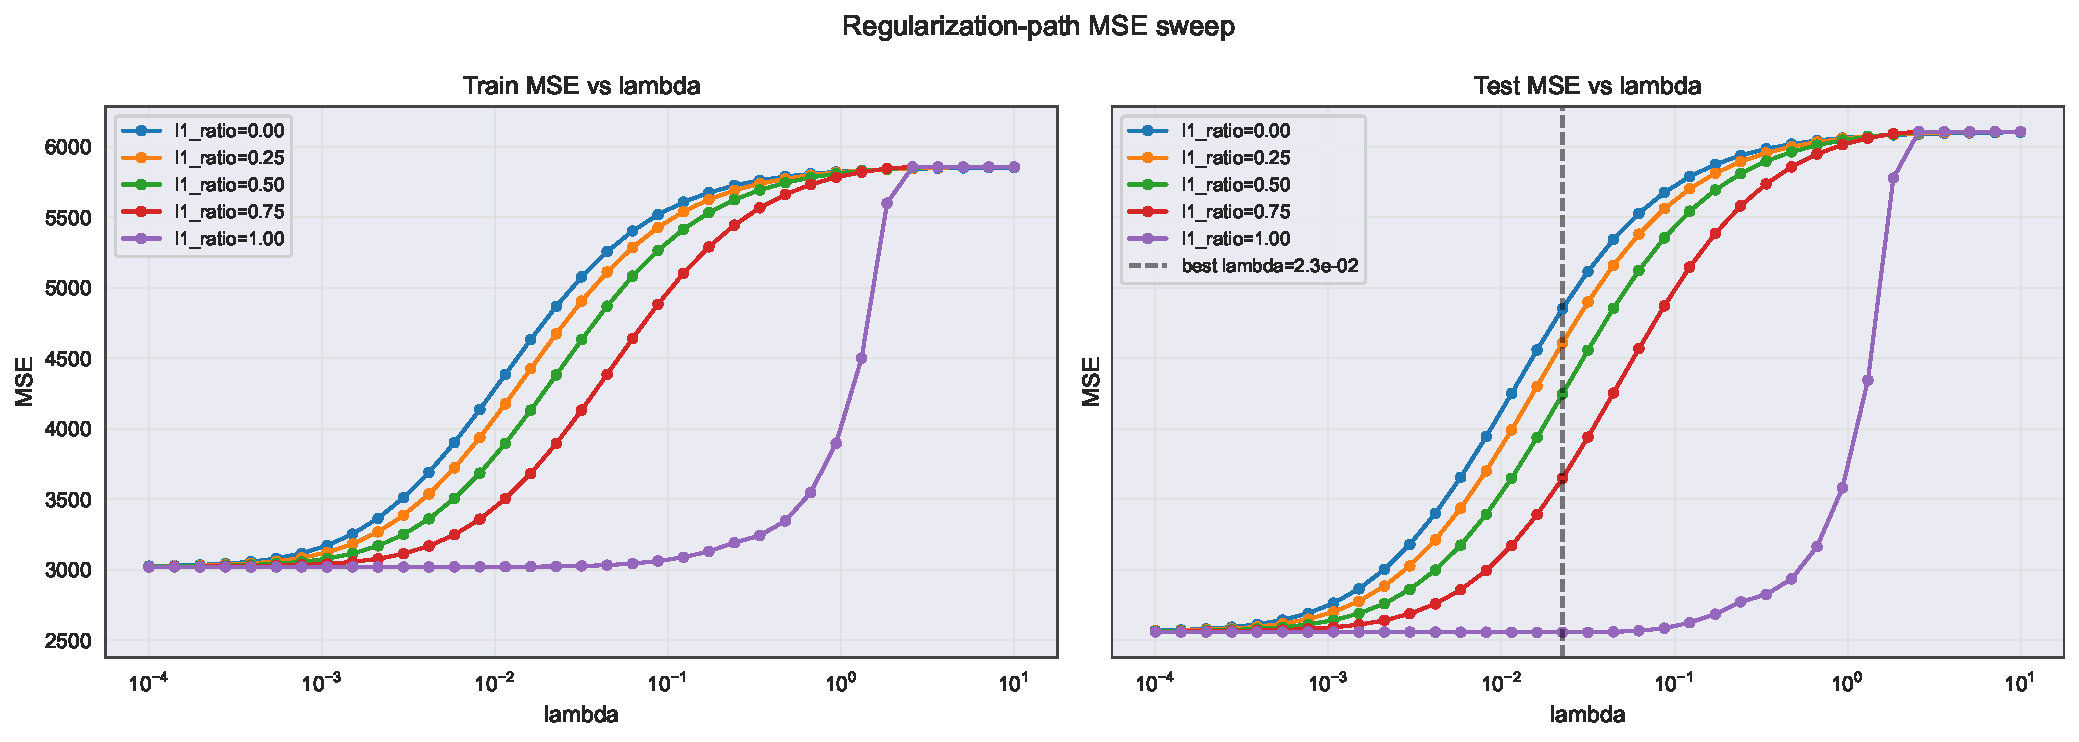
\includegraphics[width=\textwidth]{regpath_mse.pdf}
\caption{Train (left) and test (right) MSE along the regularisation path for five values of the $\ell_1$ ratio $\rho$ (\texttt{l1\_ratio} in the legend). Train MSE rises monotonically with $\lambda$. For Lasso ($\rho=1$), test MSE is essentially flat until $\lambda\approx10^{-1}$; with $\rho<1$ it rises from $\lambda\approx10^{-3}$. The dashed line marks the $\lambda$ with the lowest test MSE on the grid, shown for reference only; $\lambda$ and $\rho$ were selected by CV.}
\label{fig:regmse}
\end{figure*}

\begin{figure*}[!tp]
\centering
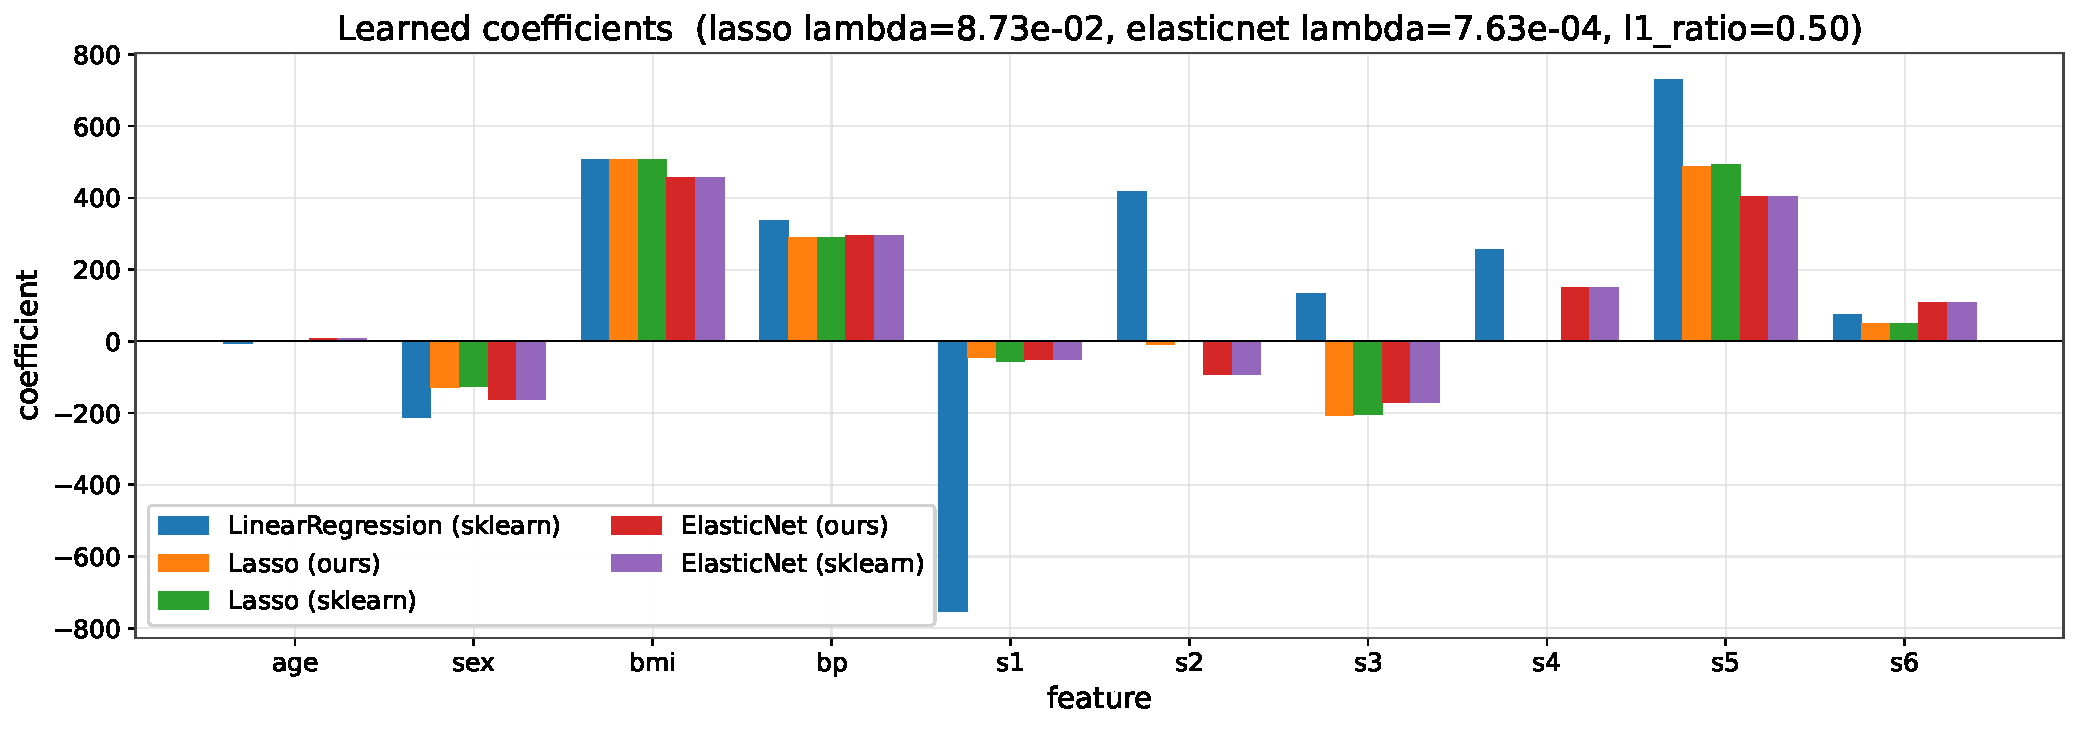
\includegraphics[width=\textwidth]{coefficient_comparison.pdf}
\caption{Learned coefficients for \texttt{LinearRegression}, our Lasso ($\lambda=0.0873$), scikit-learn's Lasso at the same $\lambda$, our ElasticNet ($\lambda=7.63\!\cdot\!10^{-4}$, $\rho=0.5$) and scikit-learn's ElasticNet at the same setting. OLS alone gives \texttt{s1} and \texttt{s2} opposing weights of magnitude $400$--$750$; both regularised models shrink the pair substantially. Our ElasticNet matches scikit-learn's to within rounding; our Lasso differs slightly on \texttt{s1} and \texttt{s2} because it has not fully converged.}
\label{fig:coefs}
\end{figure*}

\textit{Models and tuning.} We compared three predictors from scikit-learn, each retrained every January on the previous $W$ years: \texttt{Lasso}~\cite{skAPI}, which minimises~\eqref{eq:lasso}, a random forest (\texttt{RandomForestRegressor}~\cite{skRF}, RF) and an MLP (\texttt{MLPRegressor}~\cite{skAPI}). For Lasso we searched $W\in\{5,10,20\}$ and $\alpha\in\{10^{-4},10^{-3},3\cdot10^{-3},10^{-2}\}$. The random forest uses 50 trees and half of the features per split, tuned over (maximum depth, minimum leaf size) $\in\{(4,500),(8,200),(12,100)\}$. The MLP has an $\ell_2$ penalty of $10^{-3}$ and is trained with Adam for at most 30 epochs, with early stopping on 10\% of the rows (in some windows the cap ends training first); we tried hidden layers $(8)$, $(32)$ and $(32,16)$. The random forest and the MLP are trained on 200\,000 sampled rows per window. Each stock's predictions can be smoothed over time with an EWMA of half-life $h\in\{0,1,2,5,10,20\}$ days.

\textit{Design rationale.} The signal-to-noise ratio is very low (Table~\ref{tab:ic}), so overfitting is the main risk and we favour simple, stable models: six standard signals rather than a search over many candidates, which limits spurious discoveries; clipping and daily cross-sectional z-scores, so outliers and changes in overall volatility cannot dominate the fit; and small, regularised models (Lasso's $\ell_1$ penalty, the forest's large leaves and limited depth, the MLP's $\ell_2$ penalty and early stopping). Hyperparameters are chosen on 2001--2010 by validation Sharpe ratio rather than MSE (for the forest, also by holding period). The rolling window adapts to changes such as the \texttt{rev1} sign change while ten years average out the noise, demeaning the target forces the models to separate good stocks from bad ones rather than ride the market's drift, and smoothing lengthens holding periods, since fast-changing predictions are expensive to trade.

\textit{Metrics.} Each day, the predictions $\hat r_{t,i}$ are demeaned across stocks, making the portfolio market neutral in volatility-adjusted terms, and scaled so that $\sum_i|\hat r_{t,i}|=1$. The daily PnL and the annualised Sharpe ratio (benchmark zero, 252 trading days per year) are
\begin{equation}
R_t=\sum_i\tilde r_{t+1,i}\,\hat r_{t,i},\qquad \mathrm{SR}=\sqrt{252}\,\frac{\mathbb{E}[R_t]}{\sqrt{\mathrm{var}[R_t]}},
\label{eq:sharpe}
\end{equation}
The Sharpe ratio measures return per unit of risk, which is easier to interpret for trading than an MSE on noisy returns, the cumulative PnL shows whether performance is steady, and the Spearman rank correlation checks the predicted ordering of stocks while being less sensitive to extreme returns than Pearson correlation. The average holding period,
\begin{equation}
H_{av}=\frac{1}{N}\sum_{i=1}^{N}\frac{\sum_{t}|\hat r_{t,i}|}{\sum_{t}|\hat r_{t,i}-\hat r_{t-1,i}|},
\label{eq:hold}
\end{equation}
where $N$ is the number of stocks, estimates how many days positions are kept, a proxy for trading costs. Finally, the correlation of $R_t$ with an equal-weighted long-only portfolio measures how much the strategy follows the market.

\section{Results}
\subsection{Regression on Diabetes}
\label{sec:reg}

Along the Lasso path (Fig.~\ref{fig:paths}), weights reach exactly zero one at a time: \texttt{age} and \texttt{s4} first (both are zero at the CV-selected $\lambda=0.0873$) and \texttt{bmi} last ($\lambda\approx2.6$). The order does not follow the marginal correlations: \texttt{sex}, the feature least correlated with the target, outlasts \texttt{s2}, because Lasso keeps a feature for what it adds given the others. ElasticNet shrinks more gradually and zeroes weights only at larger $\lambda$. At the smallest $\lambda$, neither path has yet reached the OLS solution, for the convergence reason given below.

Train MSE rises monotonically with $\lambda$ (Fig.~\ref{fig:regmse}). For Lasso ($\rho=1$), test MSE is almost flat up to $\lambda\approx10^{-1}$ and then rises sharply as informative weights are zeroed; with any $\ell_2$ share ($\rho<1$) it rises about a hundred times earlier, from $\lambda\approx10^{-3}$. This is a scaling effect: with feature variances of about $1/442$, the penalty acts like an $\ell_1$ penalty of $21\lambda$ but an $\ell_2$ penalty of $442\lambda$ on standardised features. CV selected $\lambda=0.0873$ for Lasso (CV MSE 3335.9) and $(\lambda,\rho)=(7.63\!\cdot\!10^{-4},\,0.5)$ for ElasticNet (CV MSE 3318.0).

OLS has the lowest test MSE (2538.7), with Lasso (2586.0) and ElasticNet (2611.8) close behind, all explaining 57--58\% of the test variance (Table~\ref{tab:reg}). CV slightly preferred the penalised models, but differences under 3\% are small compared with the sampling noise of 133 test patients. OLS necessarily has the lowest training MSE, and since it also wins on the test set, ten features and 309 rows evidently leave it little room to overfit. The value of regularisation is interpretability. OLS splits the correlated pair \texttt{s1}--\texttt{s2} with large opposing weights ($-752.8$ and $+416.9$) and gives \texttt{s5} a weight of 729.9, whereas Lasso drops \texttt{age} and \texttt{s4} and shrinks the pair to $-45.4$ and $-7.8$, and ElasticNet to a more balanced $-49.5$ and $-91.3$ (Fig.~\ref{fig:coefs}).

\begin{figure}[!htbp]
\centering
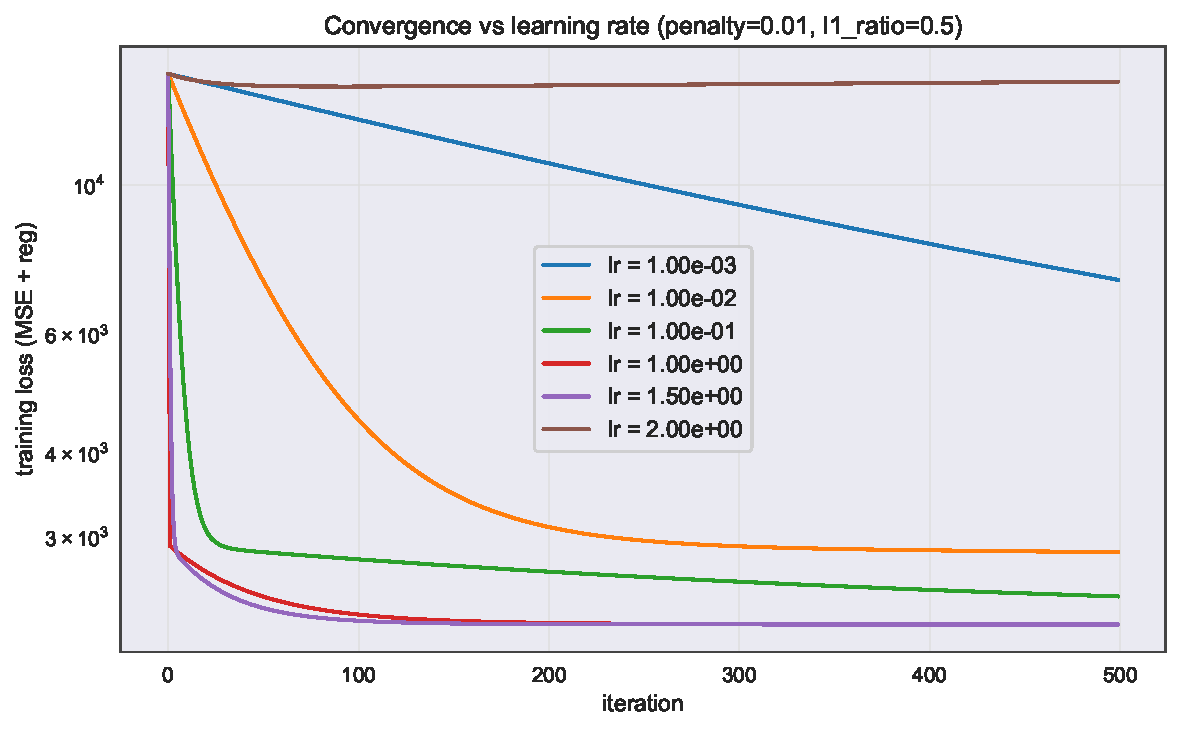
\includegraphics[width=\columnwidth]{lr_sensitivity.pdf}
\caption{Training objective of~\eqref{eq:enet} (half the MSE plus the penalty) over 500 iterations for six learning rates at $\lambda=0.01$, $\rho=0.5$. $\eta=1.5$ reaches the lowest loss. At $\eta=2$ the bias flips between 0 and $2\bar y$ every step, so the loss stays near its starting value.}
\label{fig:lr}
\end{figure}

The learning rate matters for our from-scratch models (Fig.~\ref{fig:lr}): at $\lambda=0.01$ and $\rho=0.5$, the loss decreases monotonically for every $\eta$ in $[10^{-3},\,1.5]$, with $\eta=1.5$ lowest after 500 iterations, while at $\eta=2$ the bias is on its stability limit. With nearly centred features its update is $b\leftarrow2\bar y-b$, so it flips between 0 and $2\bar y$ and the loss stays near its start.

\begin{table}[t]
\centering
\small
\caption{Diabetes regression results on the test set}
\label{tab:reg}
\setlength{\tabcolsep}{3.5pt}
\resizebox{\linewidth}{!}{%
\begin{tabular}{lcccc}
\toprule
Model & $(\lambda, \rho)$ & Train MSE & Test MSE & $R^2$\\
\midrule
LinearRegression (sklearn) & -- & \textbf{3008.7} & \textbf{2538.7} & \textbf{0.583}\\
Lasso (ours) & $(0.087,\,1)$ & 3061.8 & 2586.0 & 0.576\\
ElasticNet (ours) & $(7.6\!\cdot\!10^{-4},\,0.5)$ & 3056.2 & 2611.8 & 0.571\\
\bottomrule
\end{tabular}
}
\end{table}

\begin{figure*}[!tp]
\centering
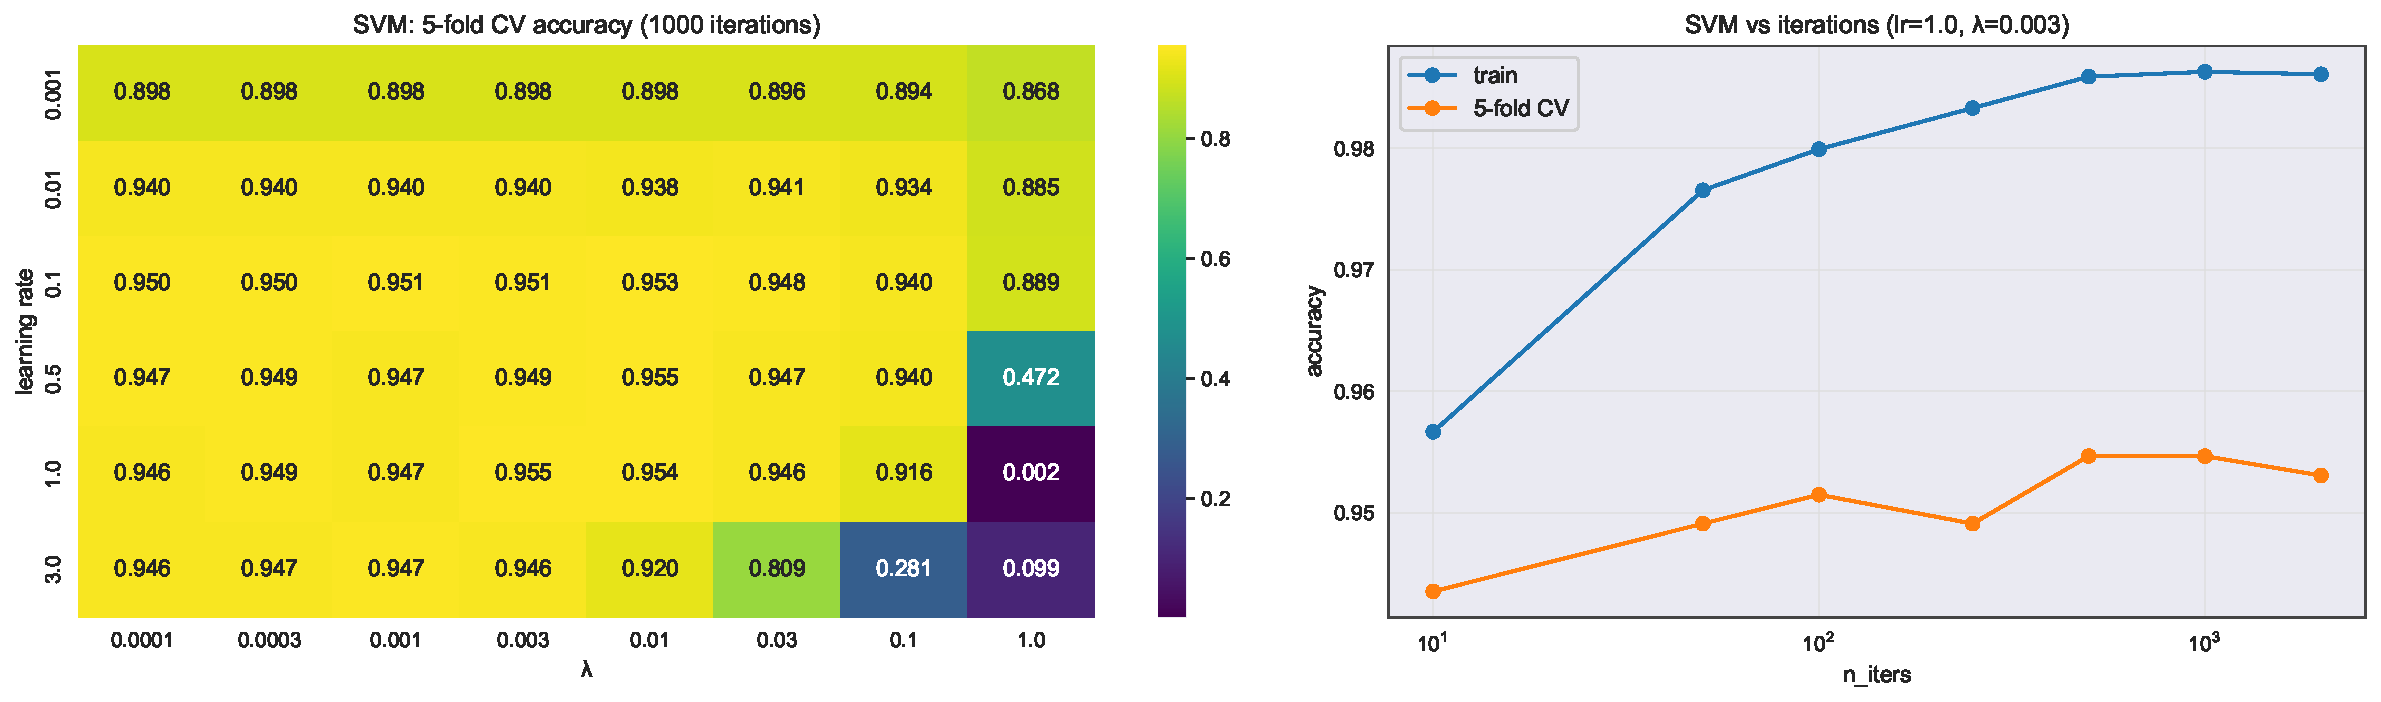
\includegraphics[width=\textwidth]{tuning_svm.pdf}\\[4pt]
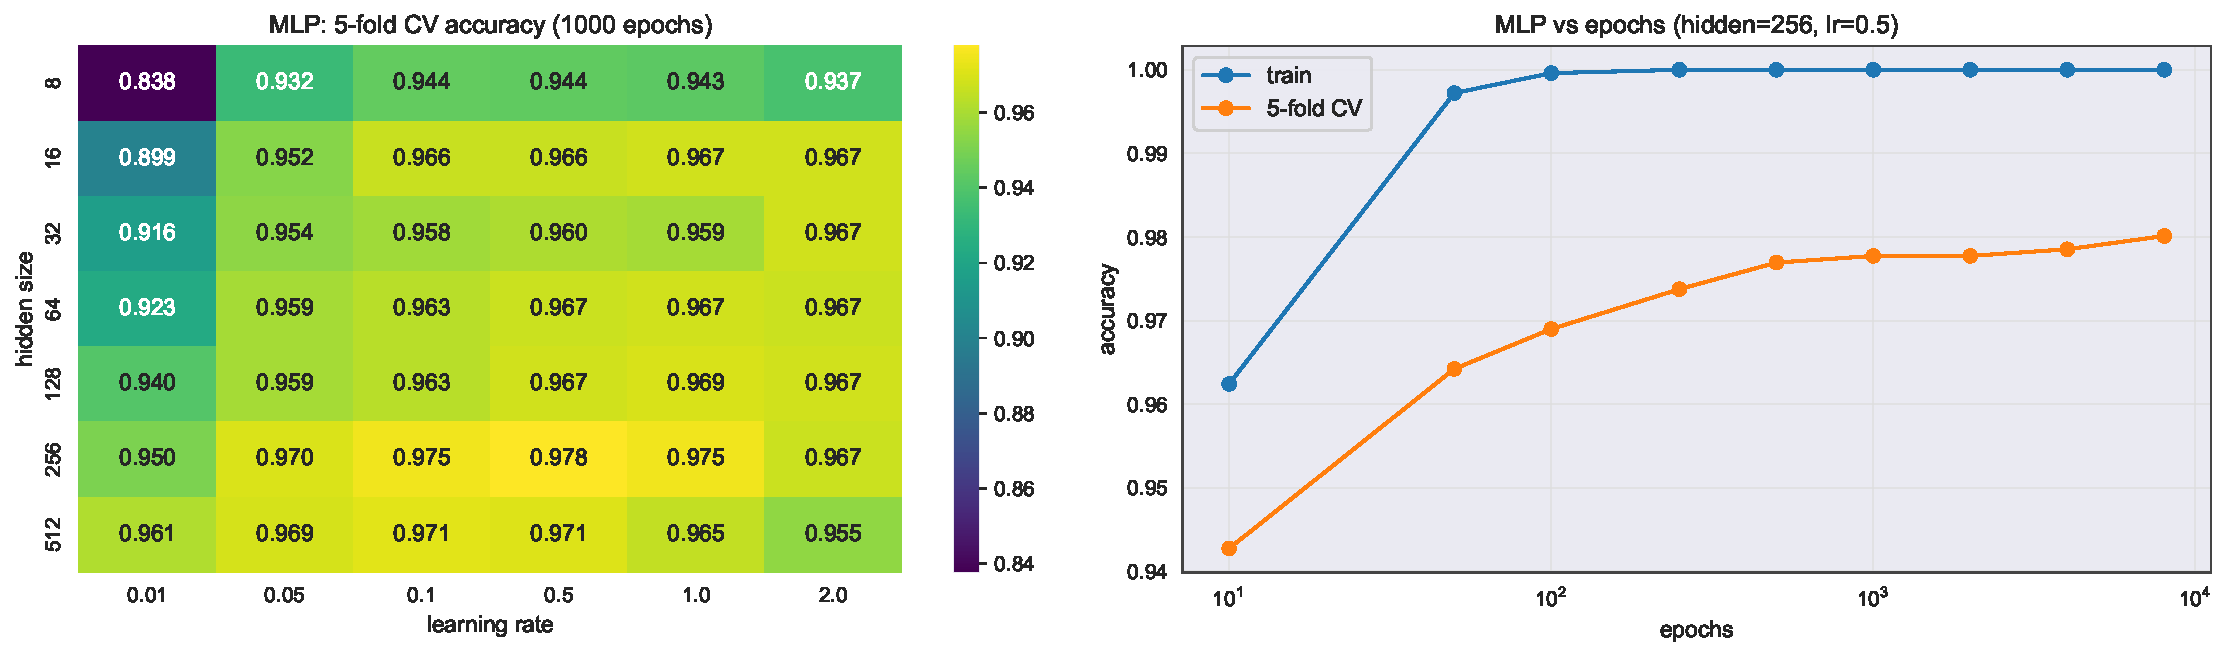
\includegraphics[width=\textwidth]{tuning_mlp.pdf}
\caption{Hyperparameter tuning of our classifiers on Digits. Top row: SVM 5-fold CV accuracy for each learning rate and $\lambda$ (left; cells below 0.86 are runs where the updates overshoot) and SVM training and CV accuracy against the number of iterations (right). Bottom row: MLP 5-fold CV accuracy for each hidden size and learning rate (left) and MLP training and CV accuracy against the number of epochs (right).}
\label{fig:tuning}
\end{figure*}

Even at $\eta=1.5$, convergence is slow in some directions. Our ElasticNet matches scikit-learn's~\cite{sklearn} to within rounding (test MSE 2611.8 for both). Our Lasso's test MSE is within 0.1\% of scikit-learn's (2586.0 against 2584.7), but its \texttt{s1}--\texttt{s2} weights differ ($-45.4$ and $-7.8$ against $-57.1$ and 0), leaving eight non-zero weights instead of seven. This is an optimisation effect: along the smallest-eigenvalue direction of $\vect{X}^\top\vect{X}/m$ ($1.9\cdot10^{-5}$), 10\,000 steps at $\eta=1.5$ remove only about a quarter of the initial error, whereas ElasticNet's $\ell_2$ term adds $\lambda(1-\rho)\approx3.8\cdot10^{-4}$ of curvature in every direction, which is enough for it to converge.

\begin{figure*}[!tp]
\centering
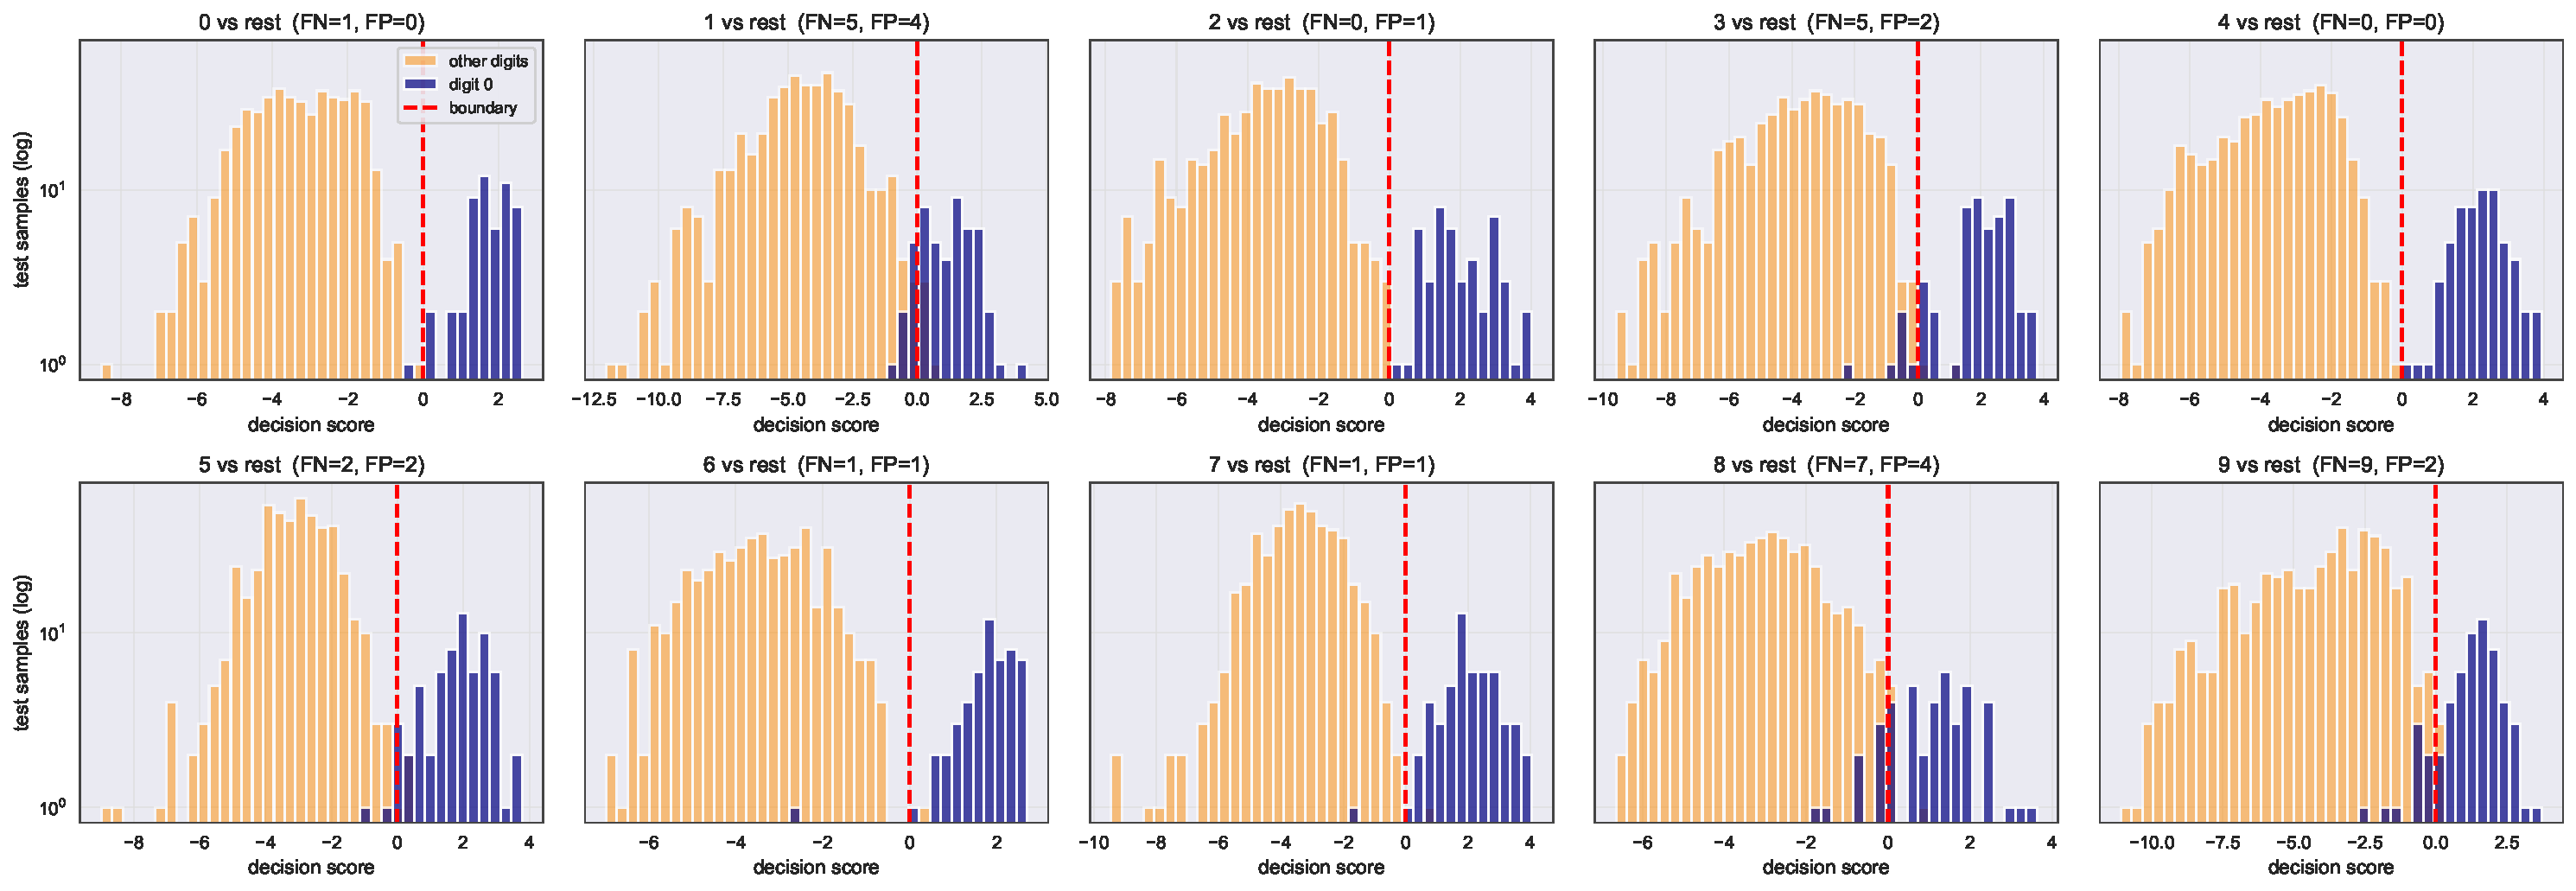
\includegraphics[width=\textwidth]{svm_scores.pdf}
\caption{SVM decision boundaries for the ten one-vs-rest classifiers. Each panel shows histograms of the test-set decision scores of the target digit (blue) and of all other digits (orange), with the counts on a log scale and the boundary $f(\mathbf{x})=0$ in red. FN\@: images of the digit scored below 0; FP\@: other digits scored above 0.}
\label{fig:svm_scores}
\end{figure*}

\begin{figure*}[!tp]
\centering
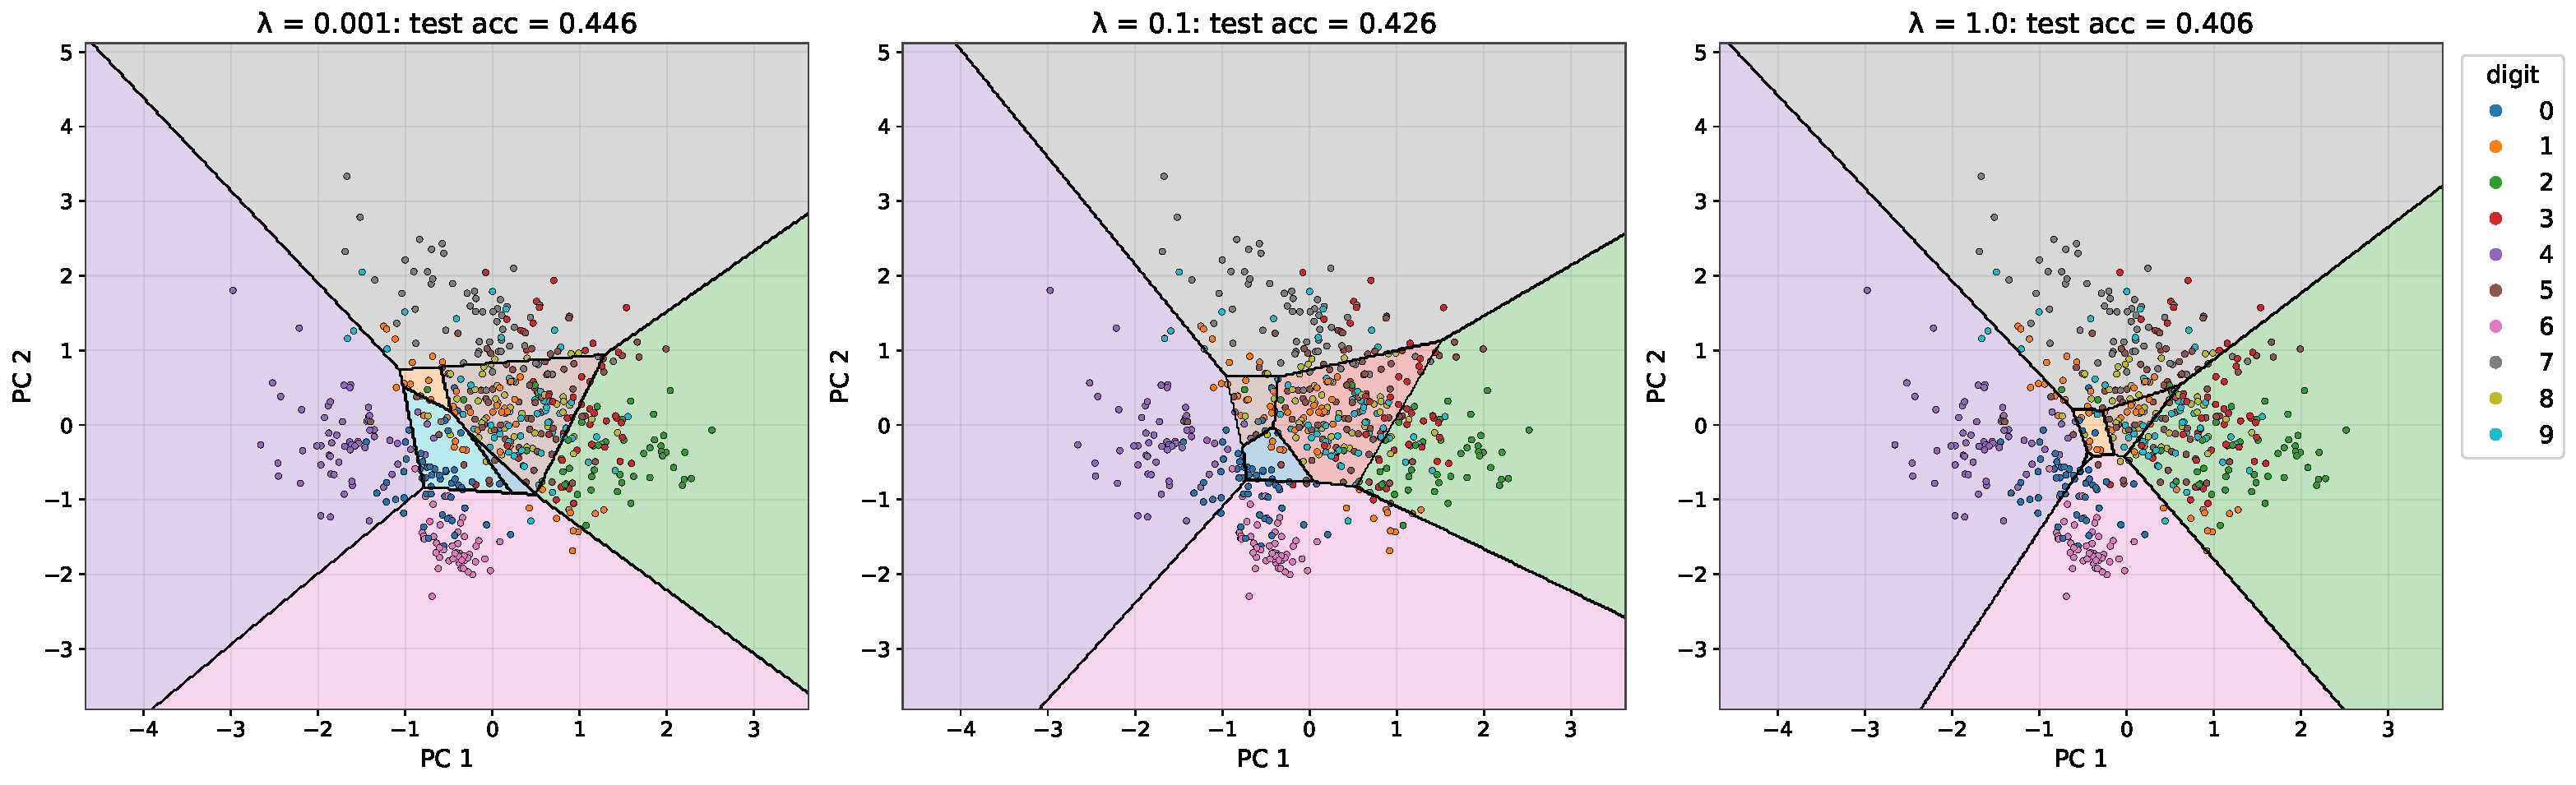
\includegraphics[width=\textwidth]{pca.pdf}
\caption{SVM decision regions in the first two principal components for $\lambda=0.001$, 0.1 and 1. Points are test samples coloured by their true digit.}
\label{fig:svm_pca}
\end{figure*}

\subsection{Classification on Digits}
\begin{table}[t]
\centering
\small
\caption{Digits classification results on the test set}
\label{tab:clf}
\setlength{\tabcolsep}{4pt}
\begin{tabular}{lcccc}
\toprule
Model & CV acc. & Train acc. & Test acc. & Errors\\
\midrule
Multiclass SVM (ours) & 0.955 & 0.983 & 0.967 & 18\\
MLP (ours) & \textbf{0.980} & 1.000 & \textbf{0.980} & \textbf{11}\\
Random forest (sklearn) & 0.975 & 1.000 & 0.970 & 16\\
\bottomrule
\end{tabular}
\end{table}

\textit{SVM.} The SVM reaches about 94--95.5\% CV accuracy over a wide range of settings (Fig.~\ref{fig:tuning}, top). It does worse when $\eta=0.001$ is too slow for 1000 iterations ($\approx0.90$), when $\lambda=1$ over-regularises (at most 0.89), and when $\eta$ and $\lambda$ are both large ($\eta\ge0.5$ with $\lambda=1$, or $\eta=3$ with $\lambda\ge0.03$), where the updates overshoot: the weight-decay step alone multiplies $\vect{w}$ by $1-2\eta\lambda$, which is 0 at $(\eta,\lambda)=(0.5,1)$ and $-1$ at $(1,1)$. The best setting, $\eta=1$, $\lambda=0.003$ and 500 iterations, gave 96.7\% test accuracy (Table~\ref{tab:clf}); the loss converged within about 100 iterations.

Fig.~\ref{fig:svm_scores} shows the test-set score $f_c(\vect{x})=\vect{w}_c^\top\vect{x}+b_c$ of each one-vs-rest classifier against its boundary $f_c(\vect{x})=0$. Digits 0, 2, 4, 6 and 7 are almost perfectly separated (at most two mistakes each), while 1, 3, 8 and 9 overlap the boundary the most, and 8 and 9 have 11 misclassified test images each. The multiclass prediction still gets most of these right, because it picks the highest score rather than requiring a positive one.

To see the boundaries in the input space, we retrained the SVM on the first two principal components (Fig.~\ref{fig:svm_pca}). The boundaries are straight lines, and because two components keep only 22\% of the variance, accuracy drops to 40--45\%. Digits 2, 4, 6 and 7 get large regions, digit 0 a small one near the centre, and the others overlap in the middle; a larger $\lambda$ shrinks the weights, so some small regions disappear and accuracy drops slightly.

\begin{figure*}[!tp]
\centering
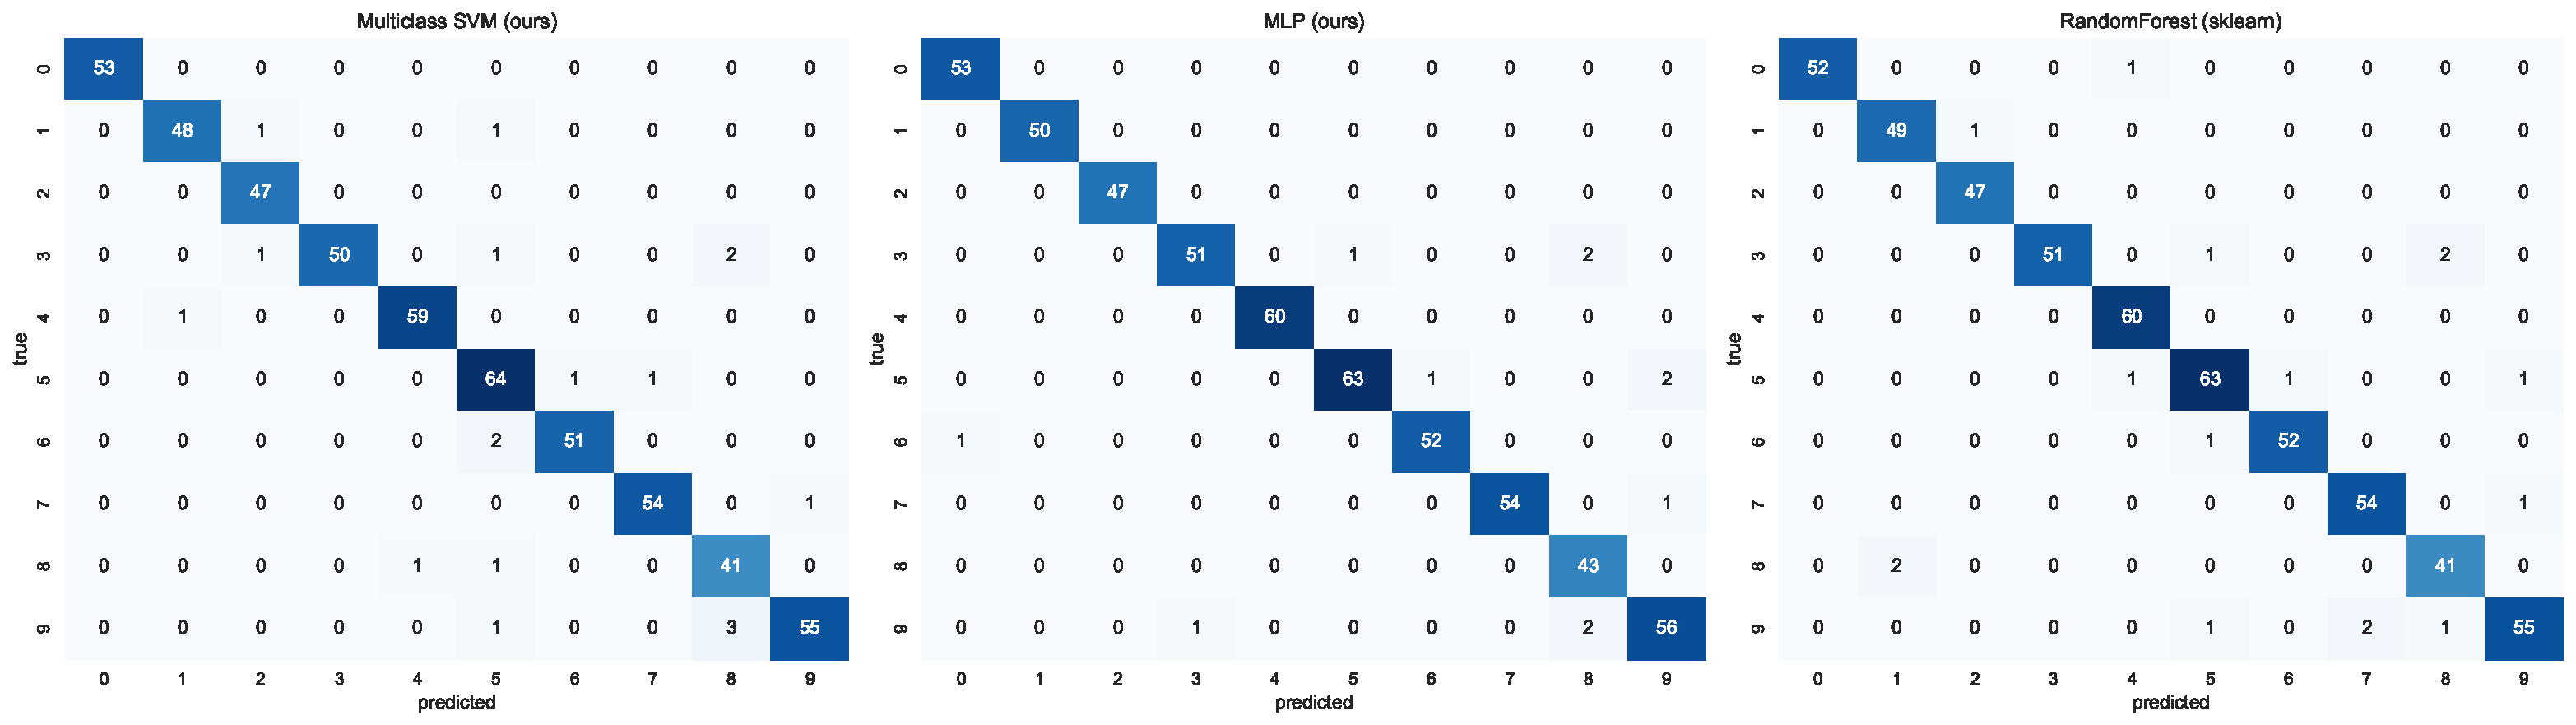
\includegraphics[width=\textwidth]{conf.pdf}
\caption{Test-set confusion matrices for the SVM (18 errors), the MLP (11) and the random forest (16). Diagonal cells are correct predictions.}
\label{fig:conf}
\end{figure*}

\textit{MLP.} Adding hidden units helps up to 256 (Fig.~\ref{fig:tuning}, bottom); $\eta=0.01$ learns too slowly, and for the larger networks $\eta=2$ starts to hurt accuracy. The best setting was $H=256$ and $\eta=0.5$. Training accuracy is essentially 100\% from about 100 epochs, but CV accuracy keeps rising slowly up to 8000 epochs, so longer training did not overfit; the final MLP, trained for 8000 epochs, reached 98.0\% test accuracy with the fewest errors of the three classifiers (Fig.~\ref{fig:conf}).

\textit{Comparison.} The best random forest used 300 trees, a maximum depth of 10, $\sqrt{n}$ features per split and a minimum leaf size of 1. On the 540 test images, the MLP makes 11 errors, the random forest 16 and the SVM 18, with the same ranking under CV (Table~\ref{tab:clf}), and most mistakes involve the digits 3, 5, 8 and 9, most often a 3 or a 9 predicted as an 8 (Fig.~\ref{fig:conf}). The SVM can only draw linear boundaries, whereas the MLP and the random forest capture non-linear patterns, which explains their small advantage.

\subsection{Return Prediction}

\textit{Tuning (2001--2010).} For Lasso, a 10-year window with $\alpha=10^{-4}$ was best (Sharpe ratio 1.51): five years seem too noisy, and twenty include relationships that no longer hold. Larger $\alpha$ removed useful features; at $\alpha=10^{-4}$, the smallest value in the grid, Lasso kept all six features with stable weights from year to year and behaved almost like least squares. For the random forest we chose depth 8 (2.68): depth 12 scored slightly higher (2.92), but its holding period fell below one day (0.95) and it was more likely to overfit. For the MLP, one hidden layer of 32 units worked best (2.43). Both non-linear models beat Lasso but held positions for only about a day.

\begin{figure}[!htbp]
\centering
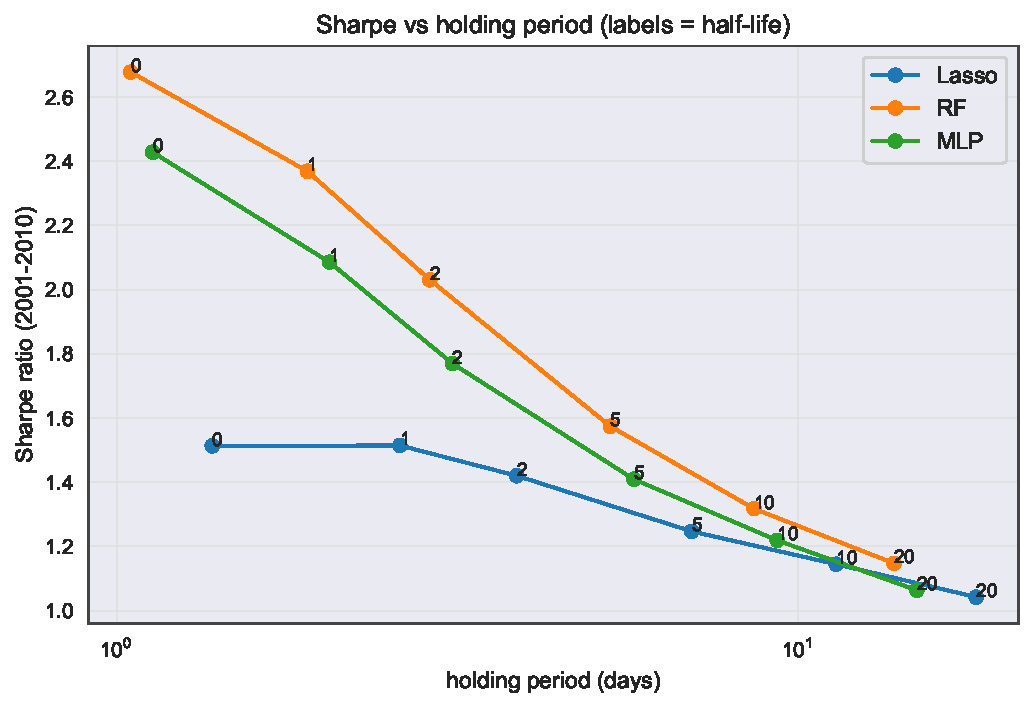
\includegraphics[width=\columnwidth]{smooth.pdf}
\caption{Validation Sharpe ratio against holding period for different smoothing half-lives $h$ (labels, in days).}
\label{fig:smooth}
\end{figure}

\textit{Smoothing.} Smoothing lengthens holding periods but lowers the Sharpe ratio, especially for the random forest and the MLP, while Lasso is less affected (Fig.~\ref{fig:smooth}). We chose $h=2$ as a compromise.

\begin{figure*}[!tp]
\centering
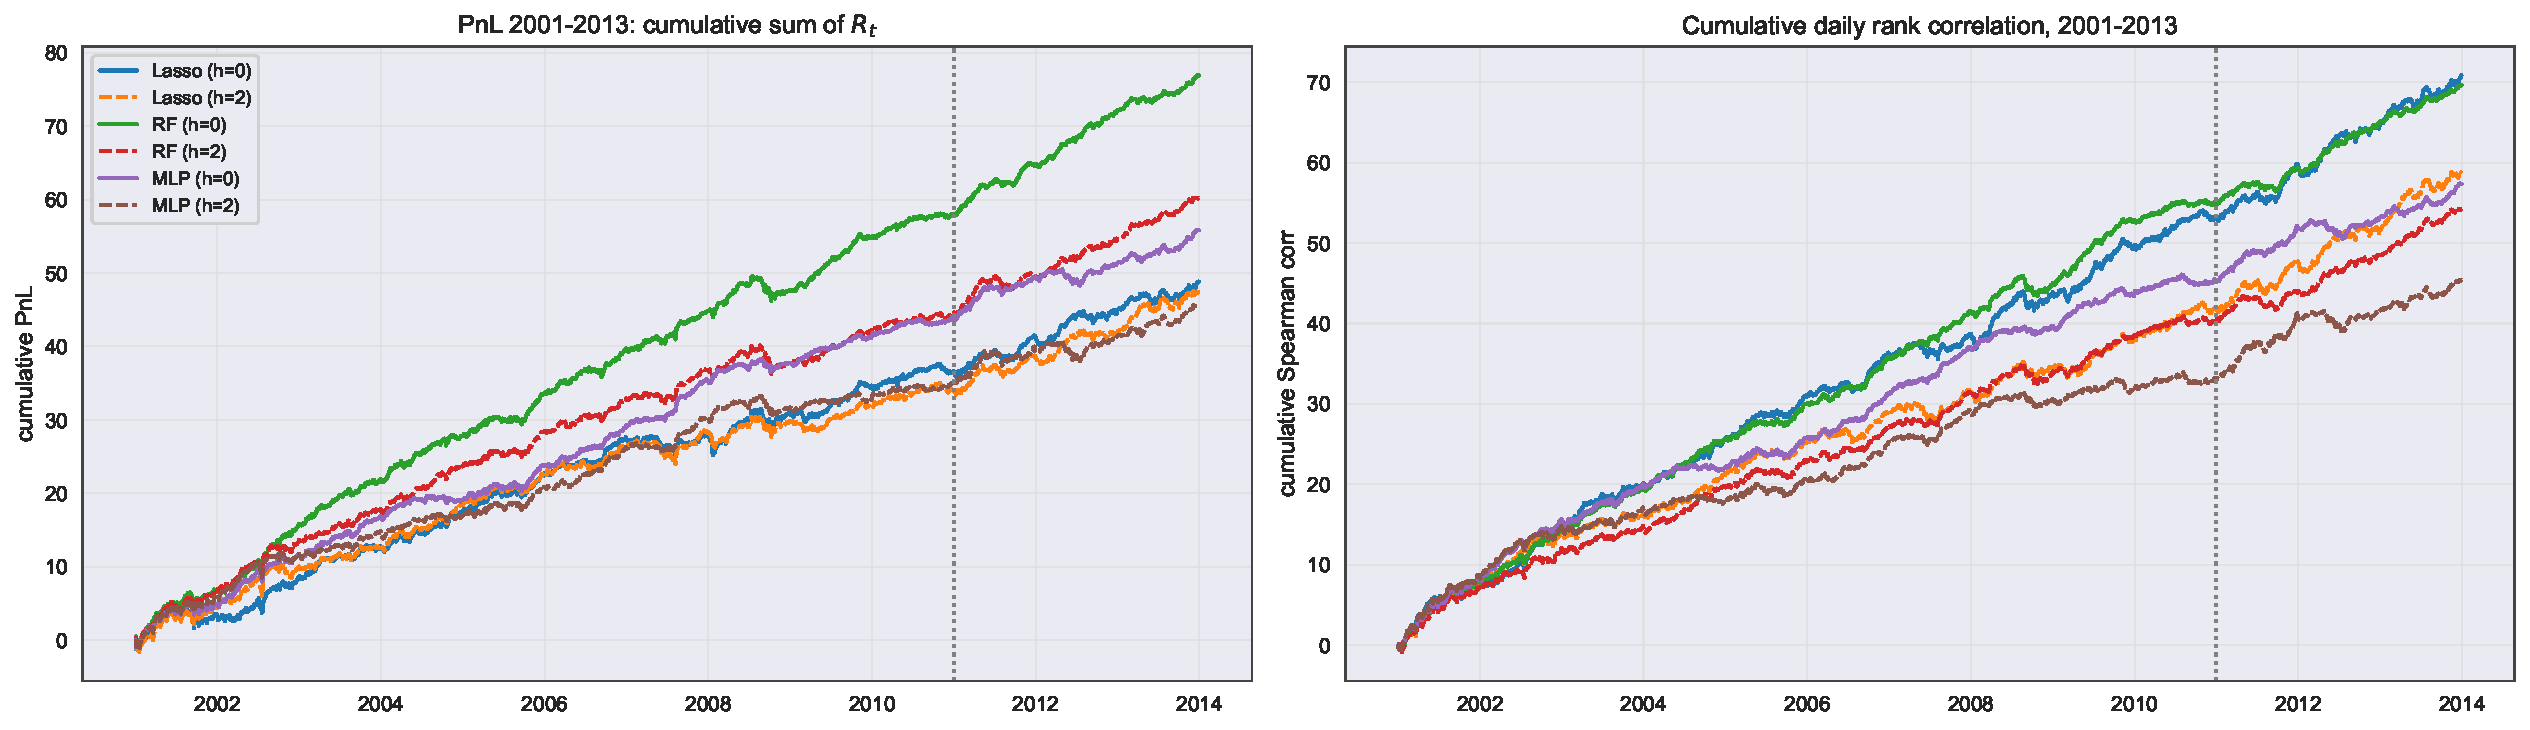
\includegraphics[width=\textwidth]{pnl.pdf}
\caption{Cumulative PnL (left) and cumulative daily rank correlation (right), 2001--2013. The dotted line marks the start of the test period. Solid lines: no smoothing; dashed lines: $h=2$.}
\label{fig:pnl}
\end{figure*}

\textit{Test results (2011--2013).} All six strategies had a positive test Sharpe ratio and predicted at least 494 stocks every day (Table~\ref{tab:test}, using~\eqref{eq:sharpe} and~\eqref{eq:hold}). The unsmoothed random forest scored highest (4.03), but its holding period of 0.90 days means its positions change by more than their own size on an average day. Smoothed Lasso offered the best balance, a Sharpe ratio of 1.96 at a 4.3-day holding period, well above the 0.8--1 the assignment calls interesting at 3--5 days. With three test years the Sharpe ratio's standard error is about $1/\sqrt{3}\approx0.58$, so even the weakest result (1.71) is clearly above zero. The market correlation (0.17--0.42) is not zero: the portfolio is neutral in volatility-adjusted terms, but the low-volatility feature favours calm stocks, which receive larger dollar positions, so the dollar exposure is slightly net long.

\begin{table}[t]
\centering
\small
\caption{Test results, 2011--2013}
\label{tab:test}
\begin{tabular}{lcccc}
\toprule
Strategy & Sharpe & Rank corr. & Hold.\ (days) & Mkt corr.\\
\midrule
Lasso, $h=0$ & 1.90 & 0.023 & 1.31 & 0.32\\
Lasso, $h=2$ & 1.96 & 0.022 & \textbf{4.26} & 0.32\\
RF, $h=0$ & \textbf{4.03} & 0.020 & 0.90 & 0.35\\
RF, $h=2$ & 2.89 & 0.018 & 2.29 & 0.42\\
MLP, $h=0$ & 2.47 & 0.016 & 1.06 & \textbf{0.17}\\
MLP, $h=2$ & 1.71 & 0.016 & 2.94 & 0.19\\
\bottomrule
\end{tabular}
\end{table}

Fig.~\ref{fig:pnl} shows that the PnL and the cumulative rank correlation rise steadily over 2001--2013, with no long losing periods, and the test years look much like the validation years. Table~\ref{tab:sub} shows that 2006--2010 was the weakest sub-period for every model except the unsmoothed MLP, whose weakest sub-period was 2001--2005. Every model had a positive Sharpe ratio in each of the 13 years, with the weakest years mostly in the 2007--2008 financial crisis.

\begin{table}[t]
\centering
\small
\caption{Sharpe ratio by sub-period (2001--2010 is validation; for $h=2$, 2011--13 differs slightly from Table~\ref{tab:test})}
\label{tab:sub}
\begin{tabular}{lcccc}
\toprule
Strategy & 2001--05 & 2006--10 & 2011--13 & 2001--13\\
\midrule
Lasso, $h=0$ & 1.83 & 1.18 & 1.90 & 1.59\\
Lasso, $h=2$ & 1.83 & 0.98 & 1.98 & 1.54\\
RF, $h=0$ & 2.89 & 2.45 & 4.03 & 2.90\\
RF, $h=2$ & 2.44 & 1.57 & 2.90 & 2.20\\
MLP, $h=0$ & 2.31 & 2.66 & 2.47 & 2.43\\
MLP, $h=2$ & 1.88 & 1.67 & 1.77 & 1.77\\
\bottomrule
\end{tabular}
\end{table}

\textit{Sentiment.} We added two Psychsignal features, net sentiment (bullish minus bearish) and activity (bullish plus bearish), each averaged over a week and set to 0 for stocks without messages. We assume each day's values are available by that day's close (otherwise another day of lag is needed, which we did not test). Because these data start in mid-2009, we retrained Lasso on up to three years of data with and without them, so the baseline differs from Table~\ref{tab:test}. Sentiment raised the test Sharpe ratio from 1.78 to 1.92 (1.52 to 1.61 with smoothing), which is not meaningful given the limited coverage and the standard error of about 0.58.

\section{Discussion and Conclusion}
On Diabetes, OLS barely overfits with ten features and 309 training points, so regularisation costs slightly more test error than it saves, and its value is interpretability. On Digits, the MLP (98.0\%) beat the random forest (97.0\%) and the linear SVM (96.7\%), so some non-linearity helps, although the linear model already performs well.

For stock returns, simple reversal, momentum and volatility features gave positive and fairly steady Sharpe ratios out of sample. The random forest and the MLP scored highest but traded almost daily, while Lasso was more stable and worked best once smoothed. The main limitations are that we ignored trading costs, which would hurt the fast strategies most, and that our grids for the non-linear models were small. In future work, we would standardise the Diabetes features so that our Lasso converges in far fewer iterations, and for the stock data add trading costs, control turnover directly, remove sector effects and test more features while guarding against false discoveries.

\section{Statement of Contributions}
Jack McDonald and William Charron-Boyle completed Tasks~1 and~2: the data analysis, the four from-scratch models and the comparison with scikit-learn. Radman Jamalshirpanjeh and Brandon Ku completed Task~3: the volatility adjustment, the features, the rolling training and evaluation, and the sentiment experiment. Each pair reviewed its own part of the notebook and wrote the corresponding sections of this report.

\textit{Use of large language models.} We used LLMs as assistants in the same ways across all three tasks. For guidance, we asked them for general advice and explanations of the tasks and equations, and consulted them on methods for testing and evaluating our models. For the code, LLMs generated our plotting code and helper functions, generated fixes for broken code, checked the notebook for bugs and helped implement the scikit-learn models. An LLM agent working on our code repository, over several prompts, merged the group members' work into the central notebook and then cleaned the repository of unused code and files. Claude also checked the notebook against the assignment several times and revised some cells (plots, markdown summaries, the data loading, the regression summary table and the lines that save the report figures as PDFs). For the report, an LLM generated the initial \LaTeX{} code, including the tables and figure layout, from our draft and helped word it in IEEE style, and Claude reviewed it against the assignment and the notebook and revised its text. All models, experiments and results come from our notebook, and we checked every number in the report.

\FloatBarrier
\begin{thebibliography}{99}
\bibitem{skAPI} scikit-learn Developers, ``API reference,'' scikit-learn documentation. Accessed: Oct. 23, 2026. [Online]. Available: \url{https://scikit-learn.org/stable/api/index.html}
\bibitem{efron} B. Efron, T. Hastie, I. Johnstone, and R. Tibshirani, ``Least angle regression,'' \emph{Ann. Statist.}, vol. 32, no. 2, pp. 407--499, 2004.
\bibitem{harris} C. R. Harris \emph{et al.}, ``Array programming with NumPy,'' \emph{Nature}, vol. 585, no. 7825, pp. 357--362, 2020.
\bibitem{sklearn} F. Pedregosa \emph{et al.}, ``Scikit-learn: Machine learning in Python,'' \emph{J. Mach. Learn. Res.}, vol. 12, pp. 2825--2830, 2011.
\bibitem{notes} M. Coates, \emph{ECSE 551: Machine Learning for Engineers, Lecture Notes} (Lectures 3, 4, 6, 7, 8 and 9), McGill University, Fall 2026.
\bibitem{tibshirani} R. Tibshirani, ``Regression shrinkage and selection via the lasso,'' \emph{J. Roy. Statist. Soc. Ser. B}, vol. 58, no. 1, pp. 267--288, 1996.
\bibitem{zou} H. Zou and T. Hastie, ``Regularization and variable selection via the elastic net,'' \emph{J. Roy. Statist. Soc. Ser. B}, vol. 67, no. 2, pp. 301--320, 2005.
\bibitem{cortes} C. Cortes and V. Vapnik, ``Support-vector networks,'' \emph{Mach. Learn.}, vol. 20, no. 3, pp. 273--297, 1995.
\bibitem{breiman} L. Breiman, ``Random forests,'' \emph{Mach. Learn.}, vol. 45, no. 1, pp. 5--32, 2001.
\bibitem{skRF} scikit-learn Developers, ``Ensembles: Random forests,'' scikit-learn User Guide. Accessed: Oct. 23, 2026. [Online]. Available: \url{https://scikit-learn.org/stable/modules/ensemble.html}
\end{thebibliography}

\end{document}